%% ------------------------------------------------------------------------- %%
%\doublespacing
\chapter{Novo Contador de N\'{u}cleos de Condensa\c{c}\~{a}o de Nuvens  - CCNC-SDCC }
\label{cap:metodologia}

%% ------------------------------------------------------------------------- %%
\PARstartOne{U}{m} novo contador de n\'{u}cleos de condensa\c{c}\~{a}o de nuvens baseado na c\^{a}mara de difus\~{a}o est\'{a}tica \'{e} proposto. Este  CCNC utiliza t\'{e}cnicas de vis\~{a}o computacional para estimar a concentra\c{c}\~{a}o de n\'{u}cleos de condensa\c{c}\~{a}o de nuvens presentes na atmosfera. O hardware do CCNC-SDCC apresentado segue uma configura\c{c}\~{a}o cl\'{a}ssica, isto \'{e}, consiste de uma c\^{a}mara com controle de diferen\c{c}a de temperatura entre as suas tampas que s\~{a}o mantidas \'{u}midas (para possibilitar a supersatura\c{c}\~{a}o de vapor de \'{a}gua no seu interior), um sistema de bomba e v\'{a}lvulas para admiss\~{a}o do ar atmosf\'{e}rico, uma fonte de luz para ilumina\c{c}\~{a}o dos aeross\'{o}is ativados (got\'{\i}culas de \'{a}gua formadas) e um sistema de medi\c{c}\~{a}o da concentra\c{c}\~{a}o de aeross\'{o}is presentes no volume de amostragem, que por sua vez \'{e} definido por uma fonte de luz, no caso um LASER do tipo HeNe.

A descri\c{c}\~{a}o do CCNC-SDCC est\'{a} dividida em duas partes: \emph{hardware} e \emph{software}. O CCNC-SDCC proposto, utiliza t\'{e}cnicas de vis\~{a}o computacional para medir a concentra\c{c}\~{a}o de aeross\'{o}is. As t\'{e}cnicas de binariza\c{c}\~{a}o por limiar e transformada \emph{watershed} s\~{a}o combinadas para medi\c{c}\~{a}o da concentra\c{c}\~{a}o dos aeross\'{o}is.

Uma metodologia inovadora para determina\c{c}\~{a}o do volume de amostragem tamb\'{e}m \'{e} apresentada. Essa metodologia dispensa a tradicional t\'{e}cnica de calibra\c{c}\~{a}o baseada na compara\c{c}\~{a}o de medi\c{c}\~{o}es com equipamentos de refer\^{e}ncia.

Nas se\c{c}\~{o}es seguintes s\~{a}o apresentados, em detalhes, o \emph{hardware}, o \emph{software}  e a metodologia de calibra\c{c}\~{a}o do volume de amostragem do CCNC-SDCC.

\section{Descri\c{c}\~{a}o do Hardware}

O principal elemento do CCNC-SDCC \'{e} a c\^{a}mara est\'{a}tica de difus\~{a}o t\'{e}rmica, conforme mostrado na Figura \ref{SDTCnova}. Como descrito no Cap\'{\i}tulo anterior, a c\^{a}mara de nuvens, deste CCNC, possui uma parede (sua parte lateral) constru\'{\i}da de um material de baixa condutividade t\'{e}rmica e imperme\'{a}vel; tampas s\~{a}o de alum\'{\i}nio (boa condutividade t\'{e}rmica) onde est\~{a}o alojados sensores de temperatura. A tampa inferior \'{e} fixa na c\^{a}mara e a tampa superior \'{e} facilmente remov\'{\i}vel para facilitar a manuten\c{c}\~{a}o interna, consistindo em remo\c{c}\~{a}o do excesso de \'{a}gua e/ou limpeza das janelas de entrada de luz LASER e filmagem. A dist\^{a}ncia entre as tampas, quando instaladas \'{e} de 1,0 cm e o interior da c\^{a}mara de nuvens \'{e} cil\'{\i}ndrico com 10,0 cm de di\^{a}metro, tendo portanto um volume interno de 78,5 $cm^{3}$. Essa c\^{a}mara possui 8 faces que facilitam a instala\c{c}\~{a}o de diversos dispositivos como por exemplo: tubos para entrada e sa\'{\i}da de ar, janelas para entrada de luz LASER, c\^{a}mera fotogr\'{a}fica digital e outros sensores caso sejam necess\'{a}rios.

\begin{figure}[!hbt]
\begin{center}
\includegraphics[scale=0.7]{eps/SDTC_nova.eps}\\
\end{center}
\caption{\label{SDTCnova}\hspace{-0.1em} desenho da nova c\^{a}mara de nuvens.}
\end{figure}

A fun\c{c}\~{a}o da c\^{a}mara de nuvens \'{e} tornar o n\'{u}cleo de condensa\c{c}\~{a}o de nuvens, admitido em seu interior, opticamente detect\'{a}vel. Isto \'{e} conseguido supersaturando com vapor de \'{a}gua o seu interior. A finalidade deste vapor \'{e} condensar sobre os aeross\'{o}is, transformando-os em got\'{\i}culas de \'{a}gua opticamente detect\'{a}veis quando iluminadas por uma fonte de luz. Para tal, uma infraestrutura de dispositivos complementam a c\^{a}mara de nuvens e que, por fim, comp\~{o}em o CCNC propriamente dito.

O diagrama esquem\'{a}tico do CCNC-SDCC \'{e} apresentado na Figura \ref{novo-ccnc}. Na parte superior (a), destacam-se a vista superior da c\^{a}mara de nuvens, uma fonte de luz LASER (635 nm), a c\^{a}mera fotogr\'{a}fica digital para o registro das imagens al\'{e}m da bomba, v\'{a}lvulas e controlador que comanda a entrada de ar atmosf\'{e}rico para o interior da c\^{a}mara de nuvens. Na parte inferior (b), destacam-se a vista lateral da c\^{a}mara de nuvens, o posicionamento das pastilhas Peltier, o papel saturado com \'{a}gua, os sensores de temperatura, o controlador PID de temperatura e o reservat\'{o}rio de \'{a}gua.

Os detalhes da c\^{a}mara de nuvens s\~{a}o mostrados em seis fotografias na Figura \ref{6figs}. Na Figura \ref{6figs} (a) \'{e} mostrada a c\^{a}mara de nuvens ainda desmontada com destaque para a lateral e para a tampa superior que \'{e} composta por dois discos de alum\'{\i}nio (tampa externa e tampa interna). Estes discos, quando juntos, acomodam entre si um tecido de algod\~{a}o, cuja finalidade \'{e} armazenar \'{a}gua no interior da tampa para que essa possa ser liberada de forma gradativa por orif\'{\i}cios igualmente espa\c{c}ados na face inferior da tampa. \'{E} importante ressaltar que um fino tecido de algod\~{a}o recobre o disco menor para garantir uma uniforme distribui\c{c}\~{a}o da \'{a}gua na superf\'{\i}cie de alum\'{\i}nio, exposta no interior da c\^{a}mara.  Na Figura \ref{6figs} (b) \'{e} mostrada a tampa superior montada, bem como a c\^{a}mara. Na Figura \ref{6figs} (c) destaca-se a c\^{a}mera fotogr\'{a}fica fixada na lateral da c\^{a}mara de nuvens. Na Figura \ref{6figs} (d) \'{e} apresentada a c\^{a}mara de nuvens e o seu reservat\'{o}rio de \'{a}gua. Por fim, na Figura \ref{6figs} (e) visualiza-se a c\^{a}mara de nuvens montada com sensores de temperatura, pastilha Peltier e o circuito eletr\^{o}nico de controle pronto para testes.




\begin{figure}[!hbt]
\begin{center}
\includegraphics[scale=0.8]{eps/novo_ccnc2.eps}\\
\end{center}
\caption{\label{novo-ccnc}\hspace{-0.1em} diagrama esquem\'{a}tico do novo CCNC.}
\end{figure}





\begin{figure}%
\centering
\subfigure[lateral da c\^{a}mara e detalhes da tampa superior.]{\label{sdccDet1}\includegraphics[scale=0.1]{eps/ccnc_detalhes_1a.eps}} %
\subfigure[tampa superior e a c\^{a}mara montadas.]{\label{sdccDet2}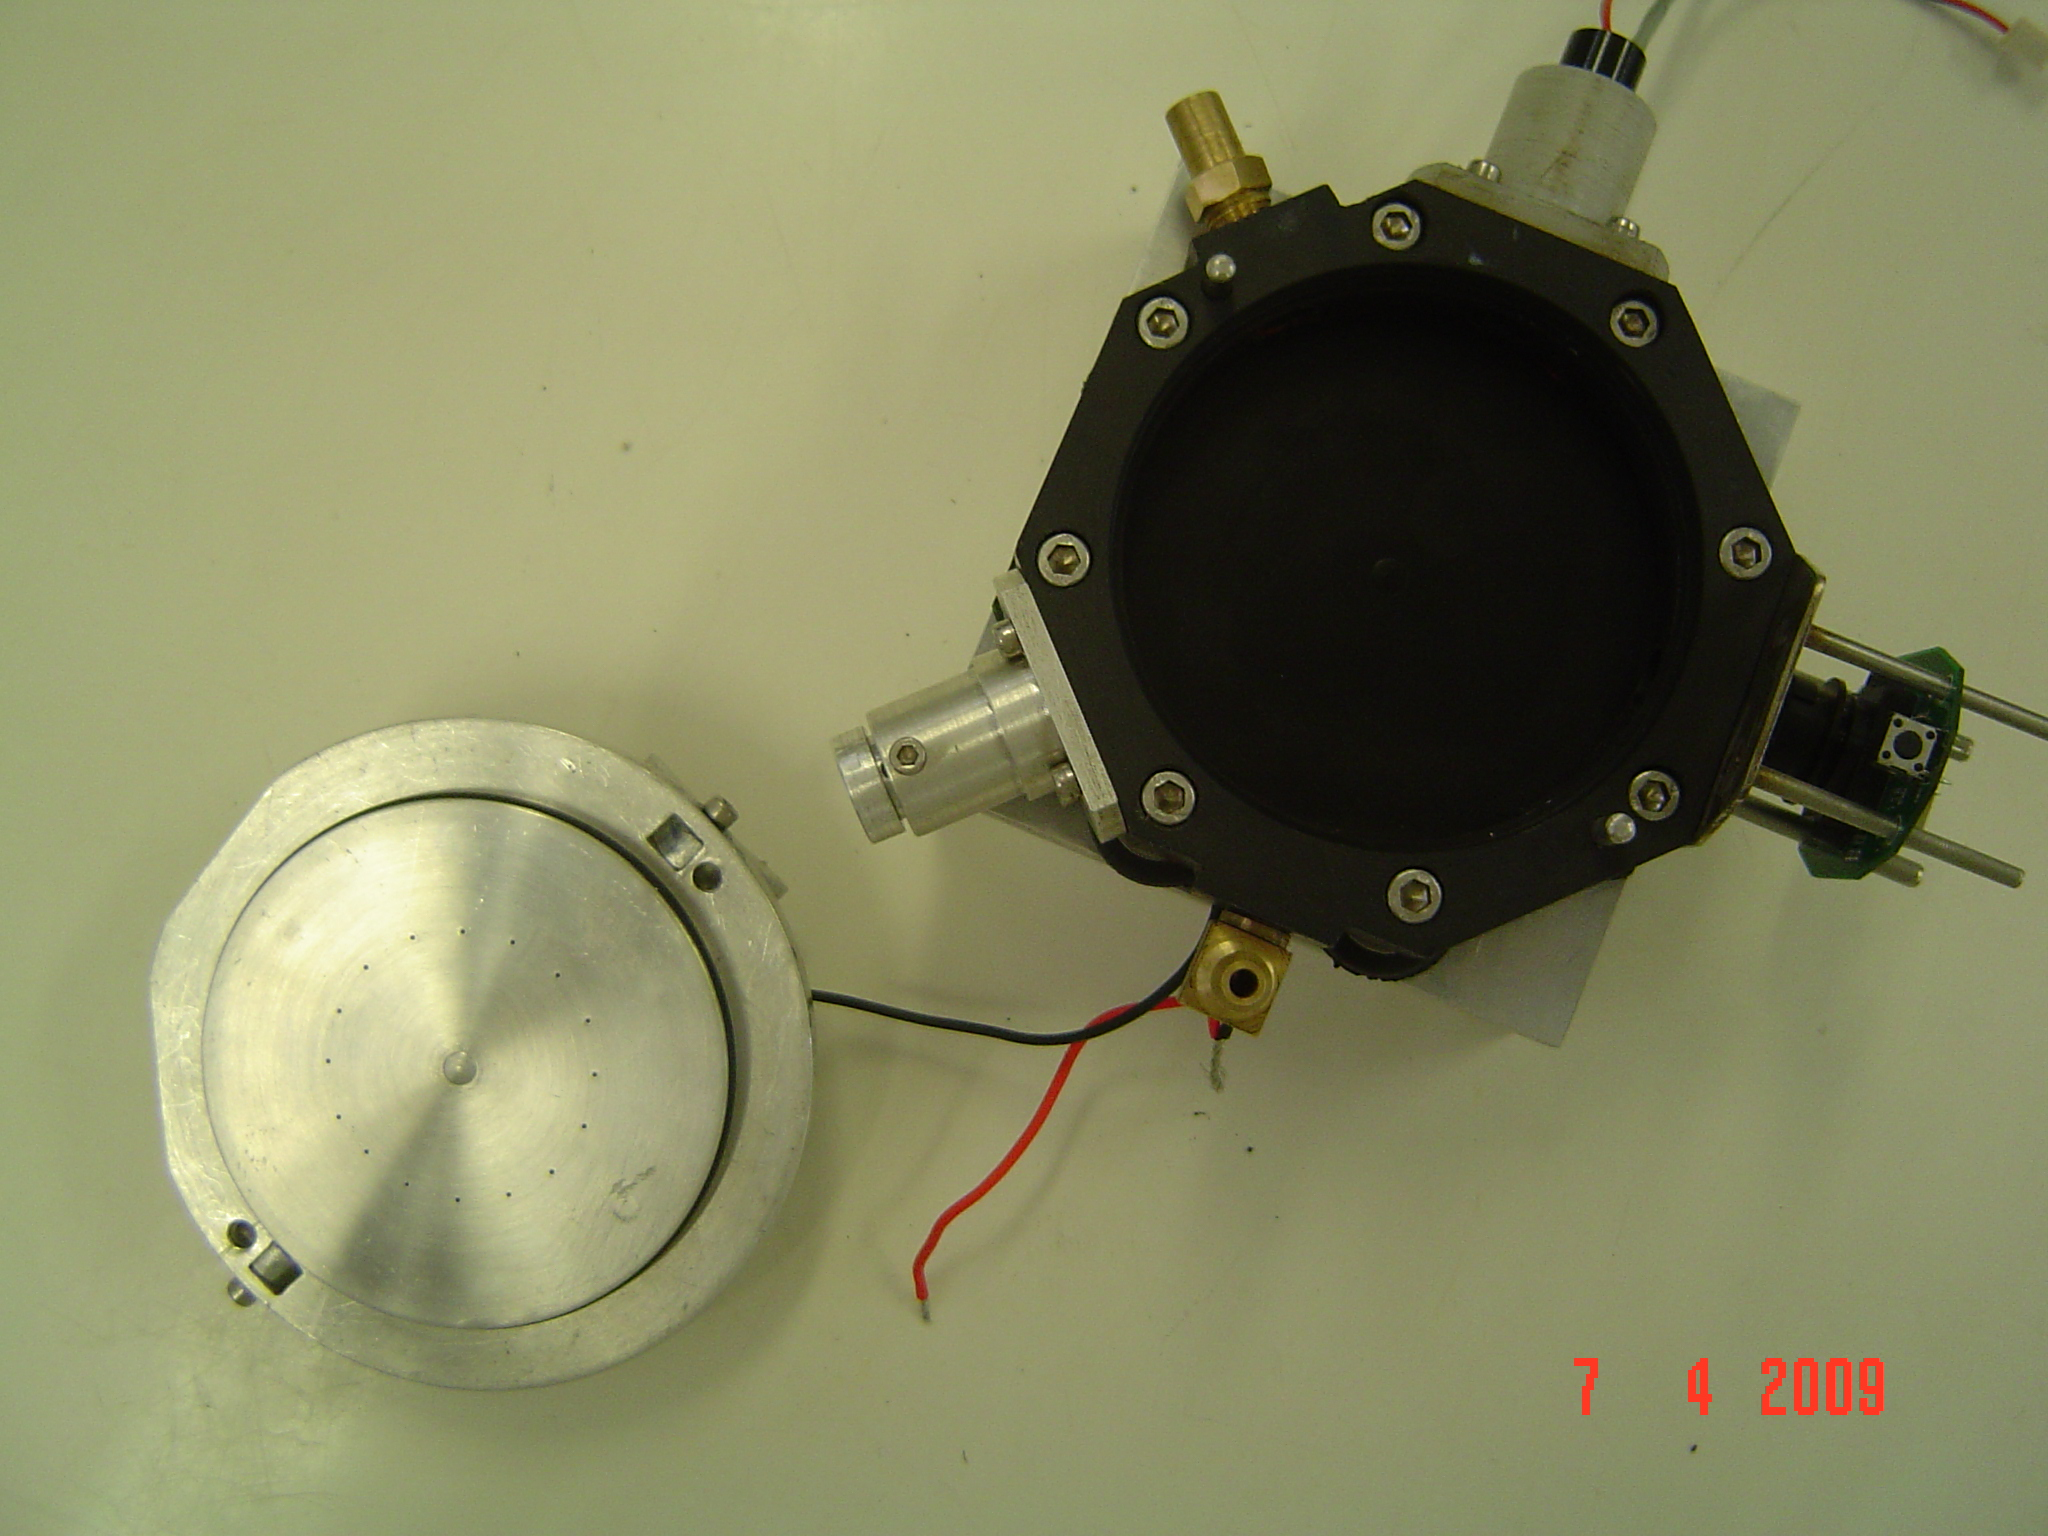
\includegraphics[scale=0.1]{eps/ccnc_detalhes_2.eps}} \\
\subfigure[WEBCAN fixada na lateral da c\^{a}mara.]{\label{sdccDet3}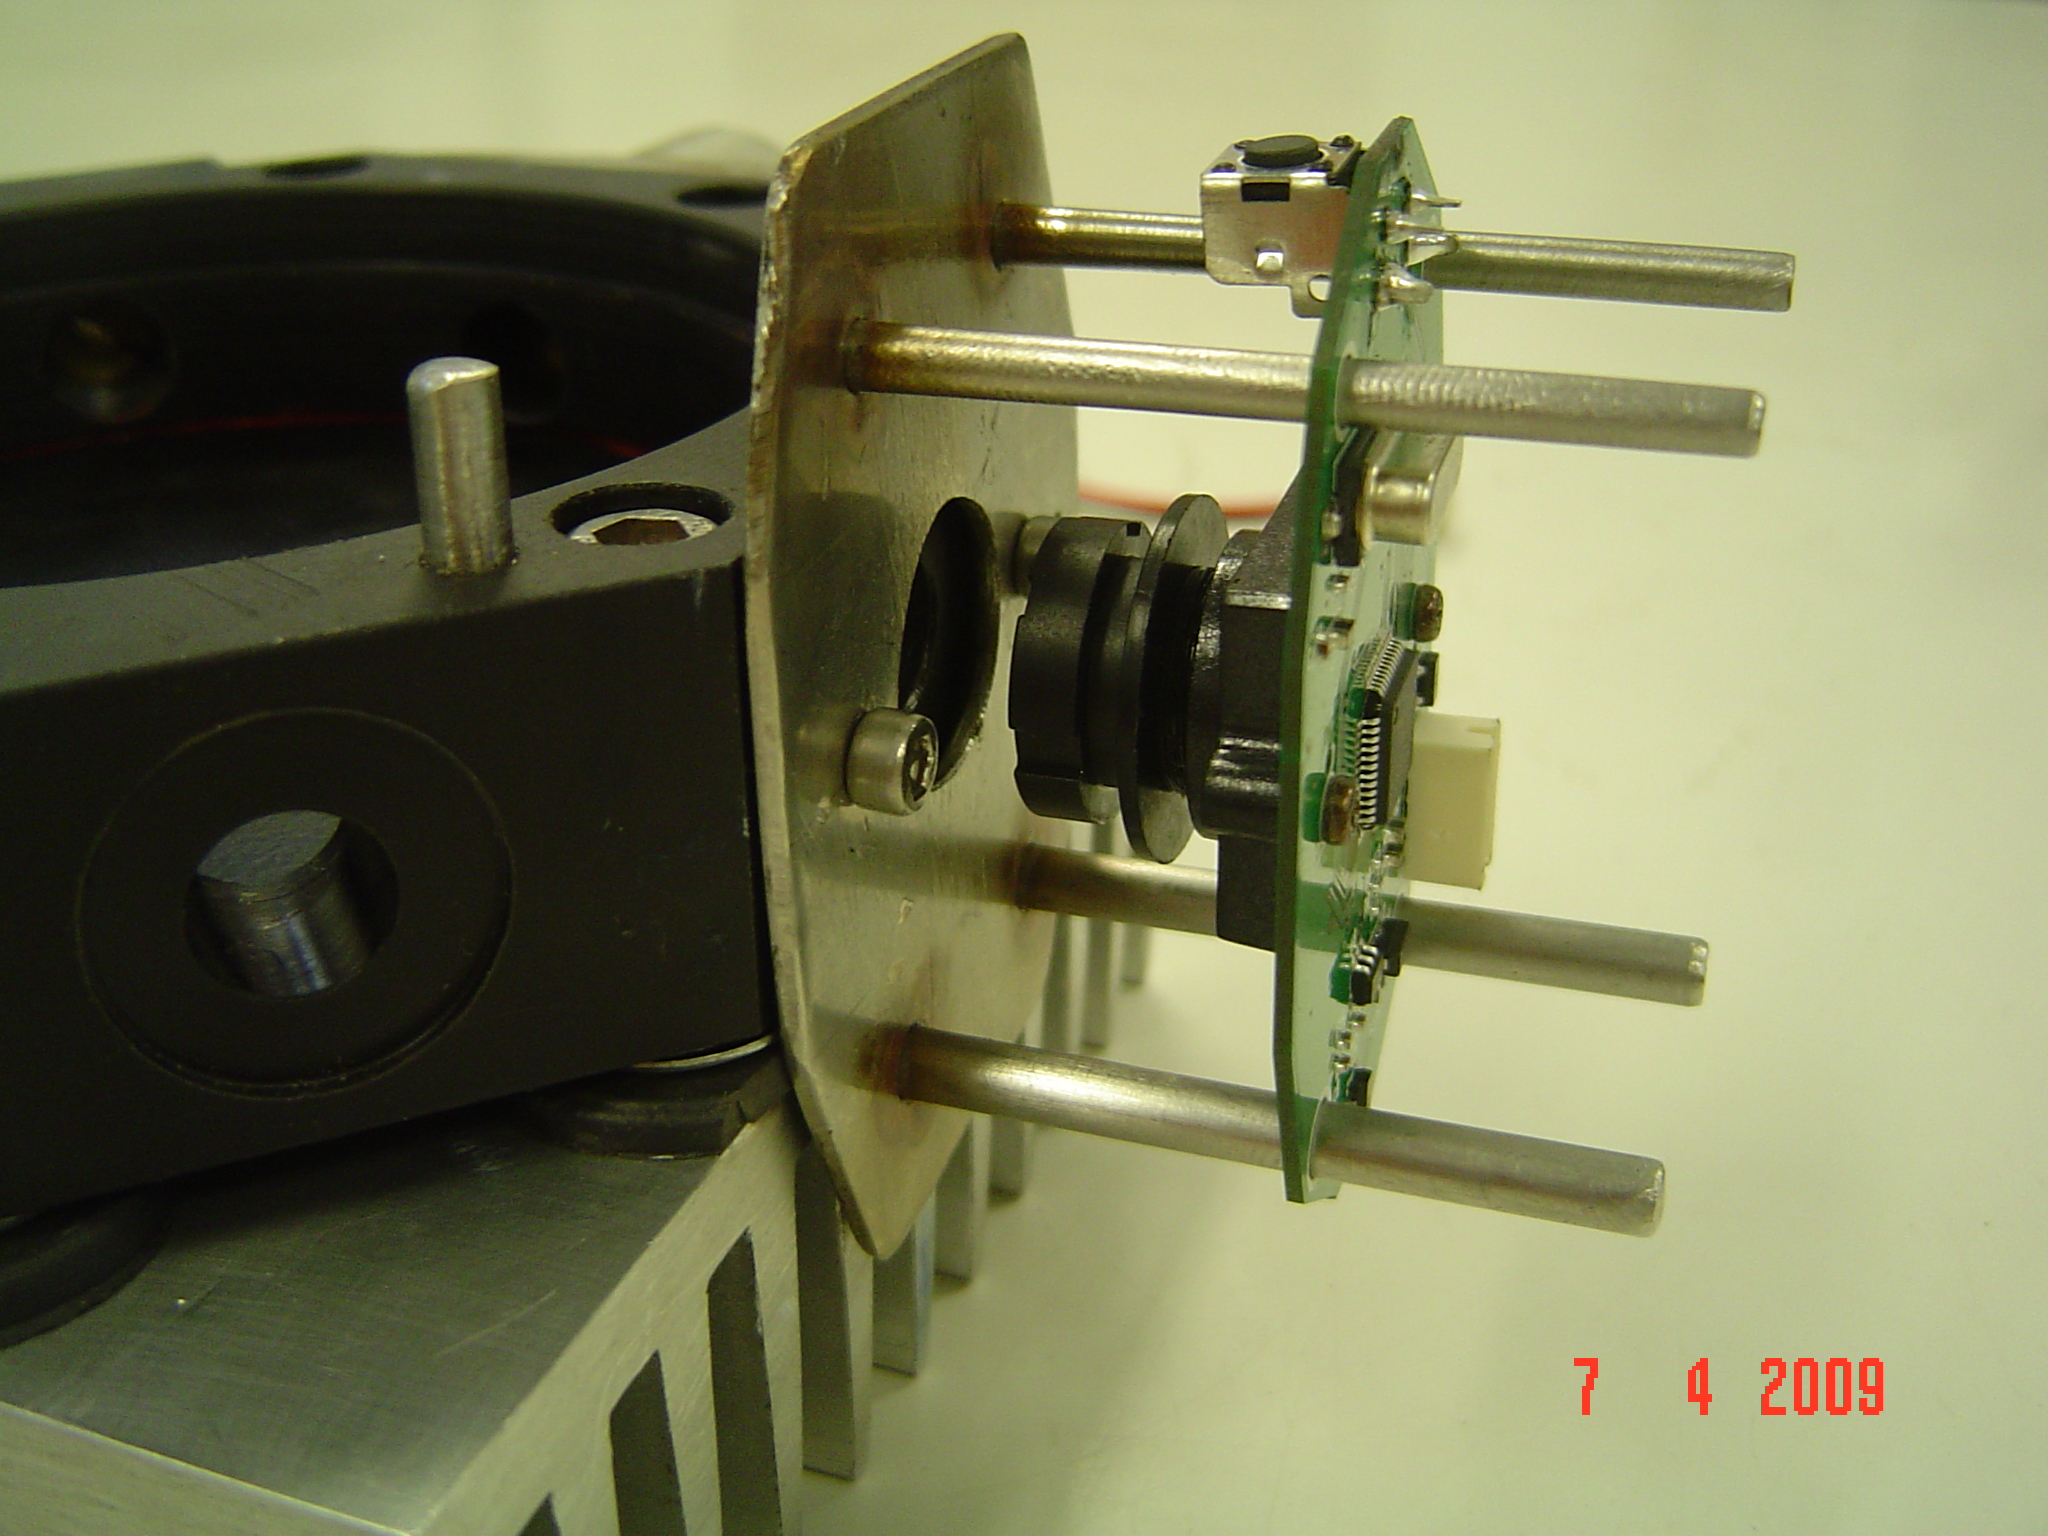
\includegraphics[scale=0.1]{eps/ccnc_detalhes_3.eps}} %
\subfigure[c\^{a}mara montada e o reservat\'{o}rio de \'{a}gua.]{\label{sdccDet4}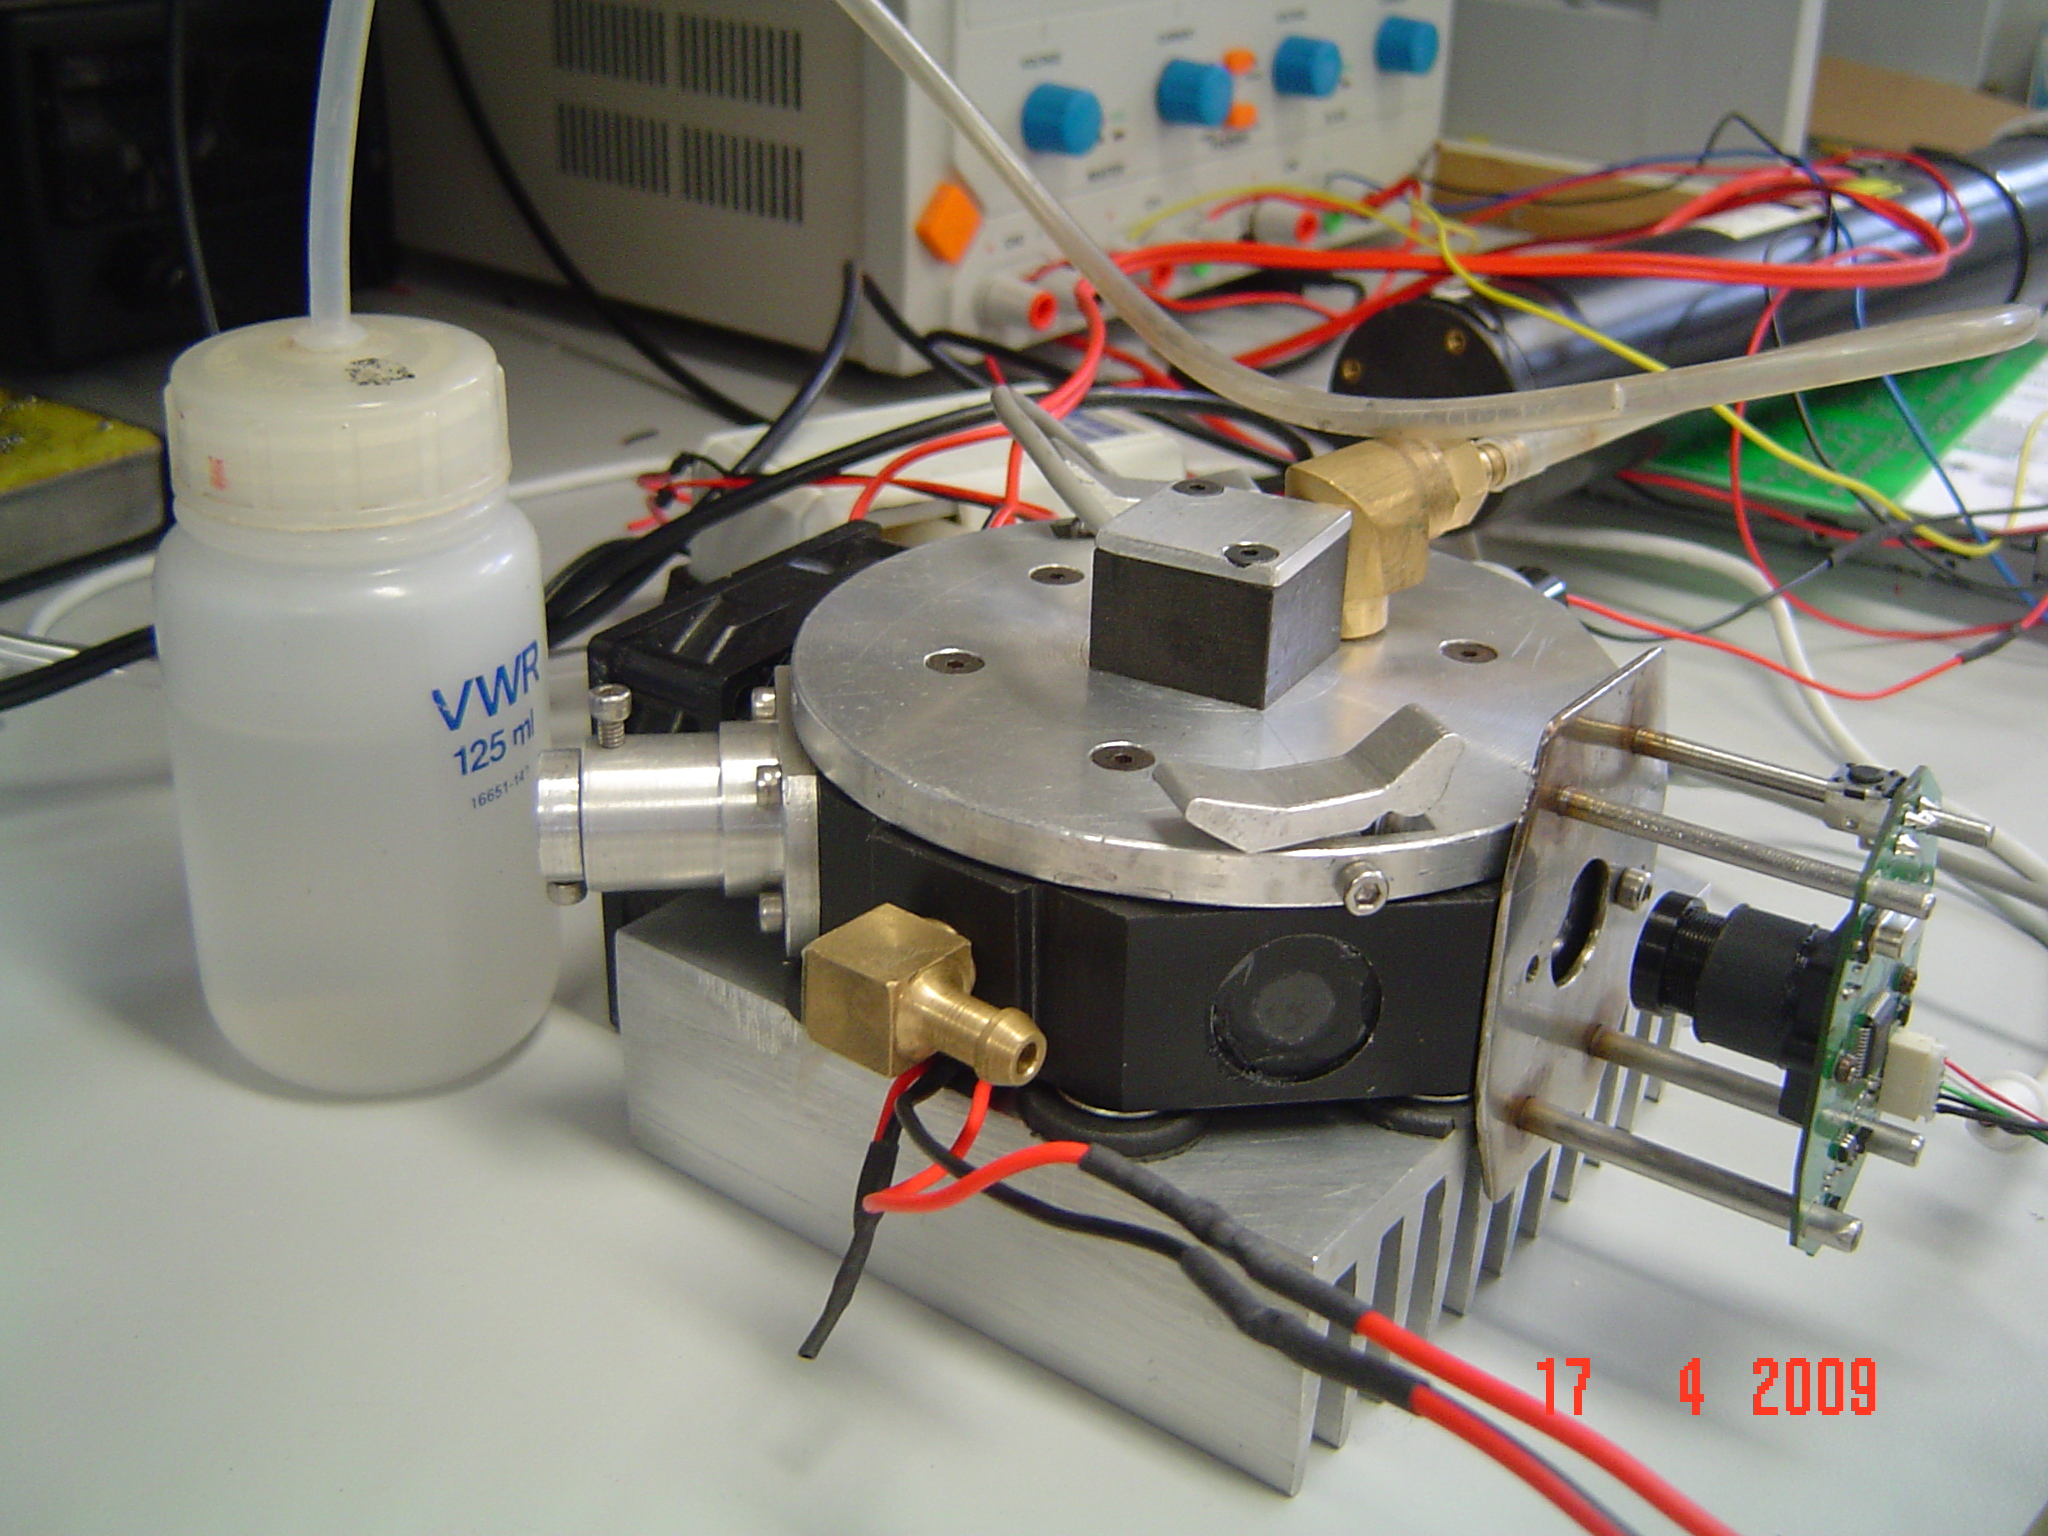
\includegraphics[scale=0.1]{eps/ccnc_detalhes_4.eps}} \\

%\subfigure[detalhes]{\label{sdccDet5}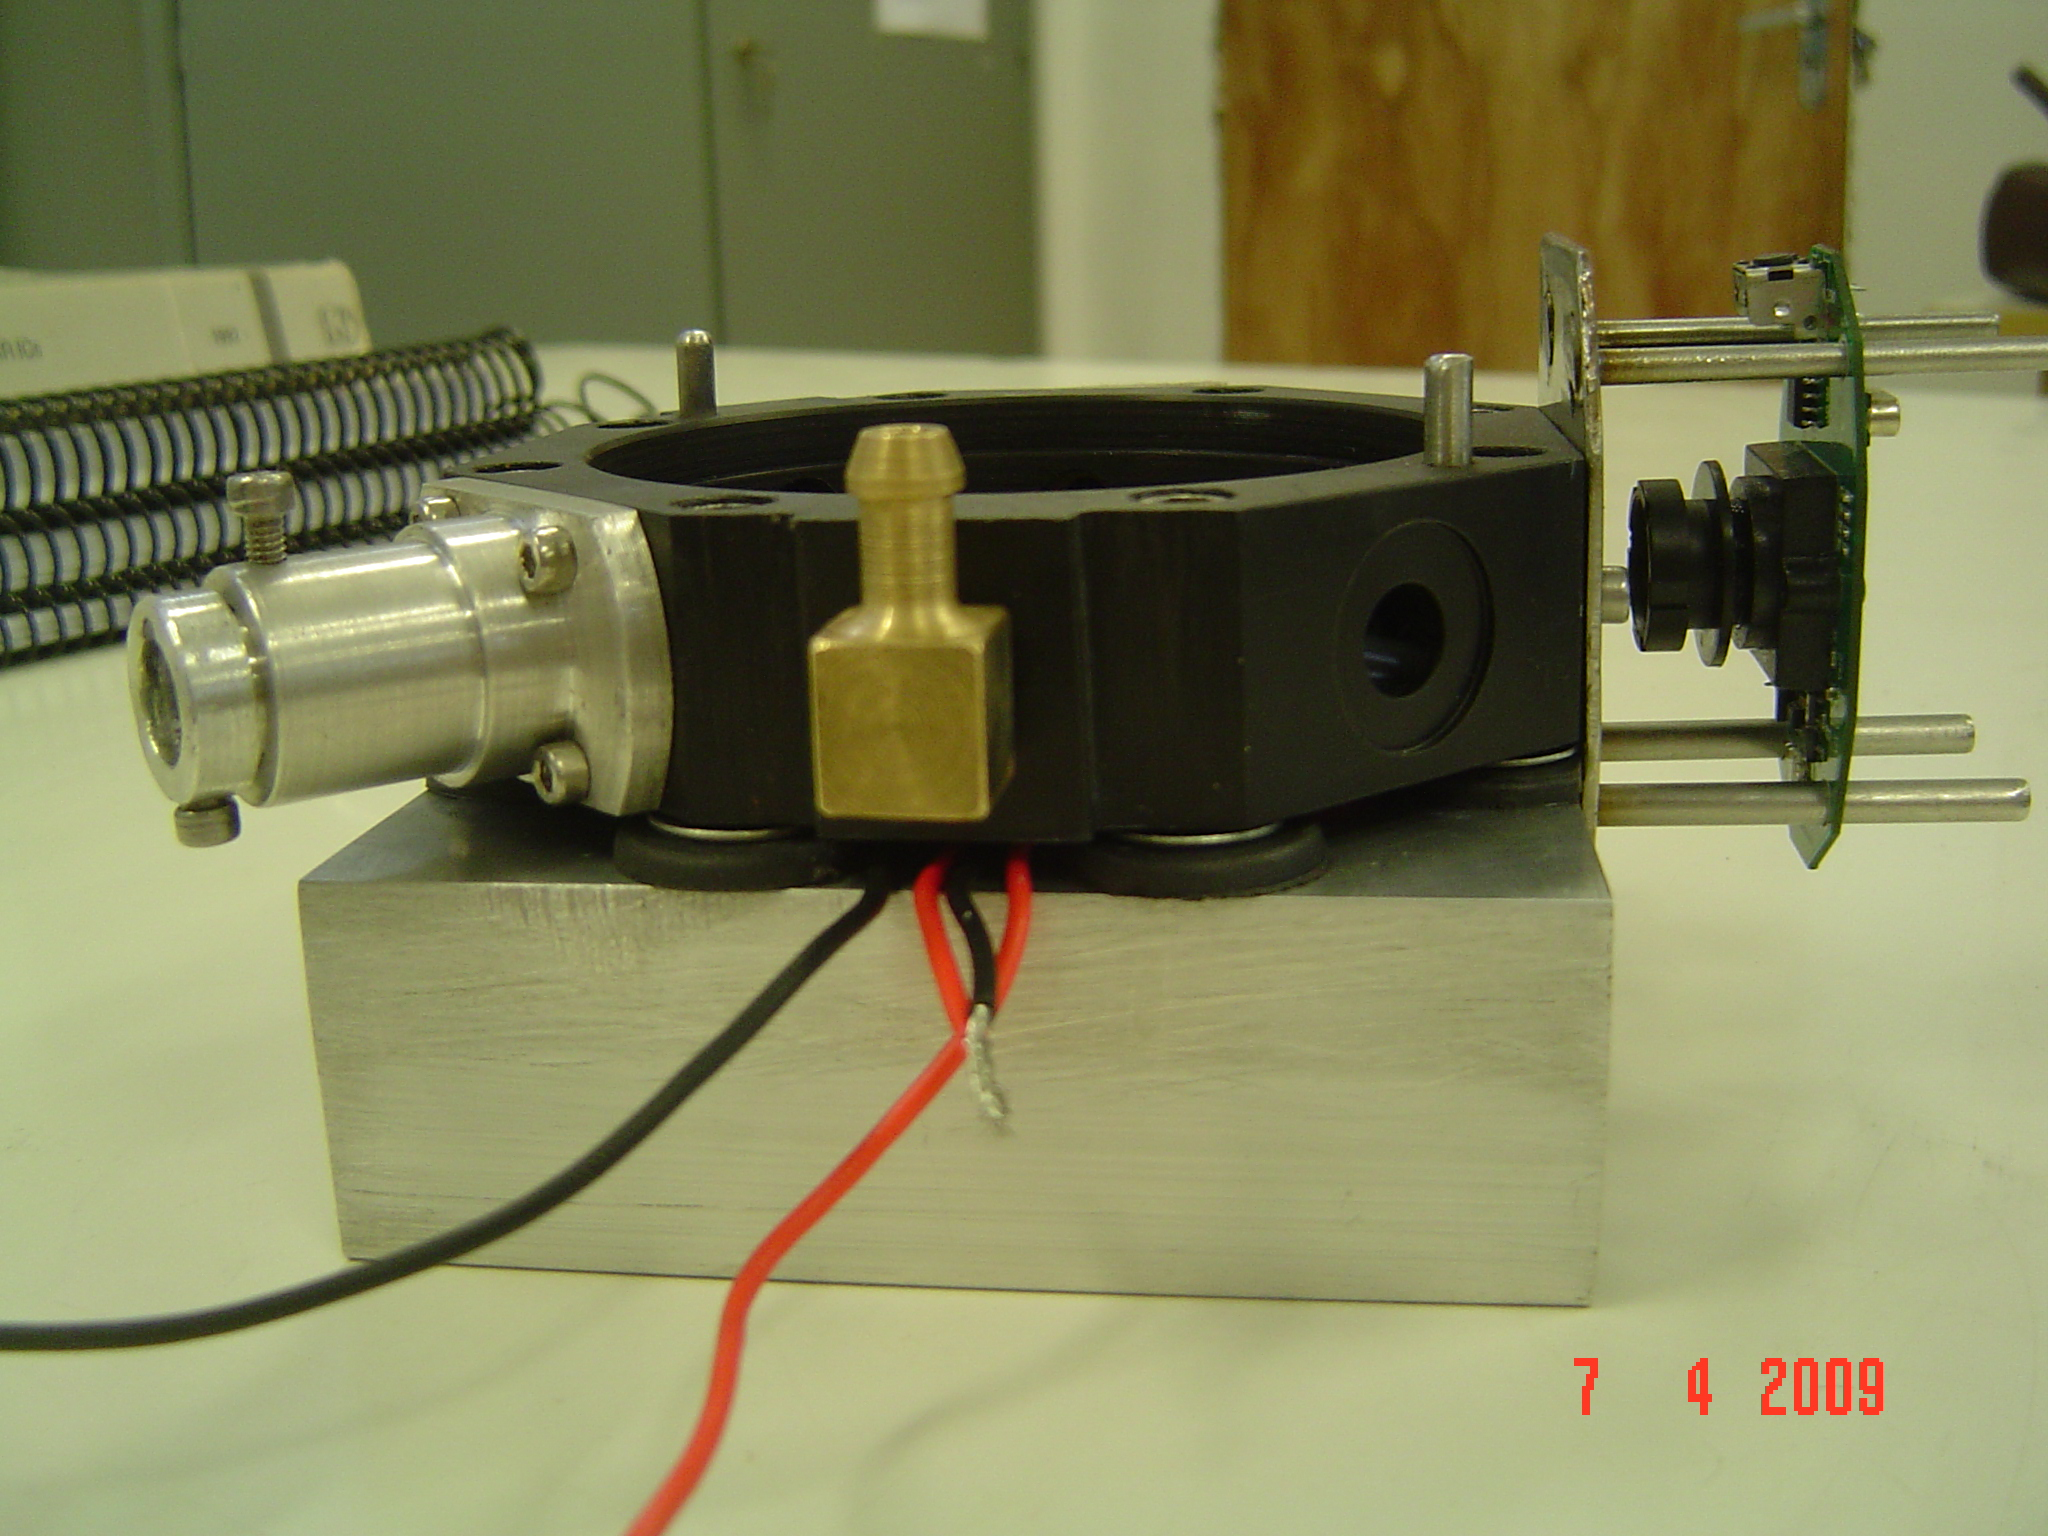
\includegraphics[scale=0.1]{eps/ccnc_detalhes_5.eps}} %
\subfigure[a c\^{a}mara e o circuito eletr\^{o}nico de controle.]{\label{sdccDet6}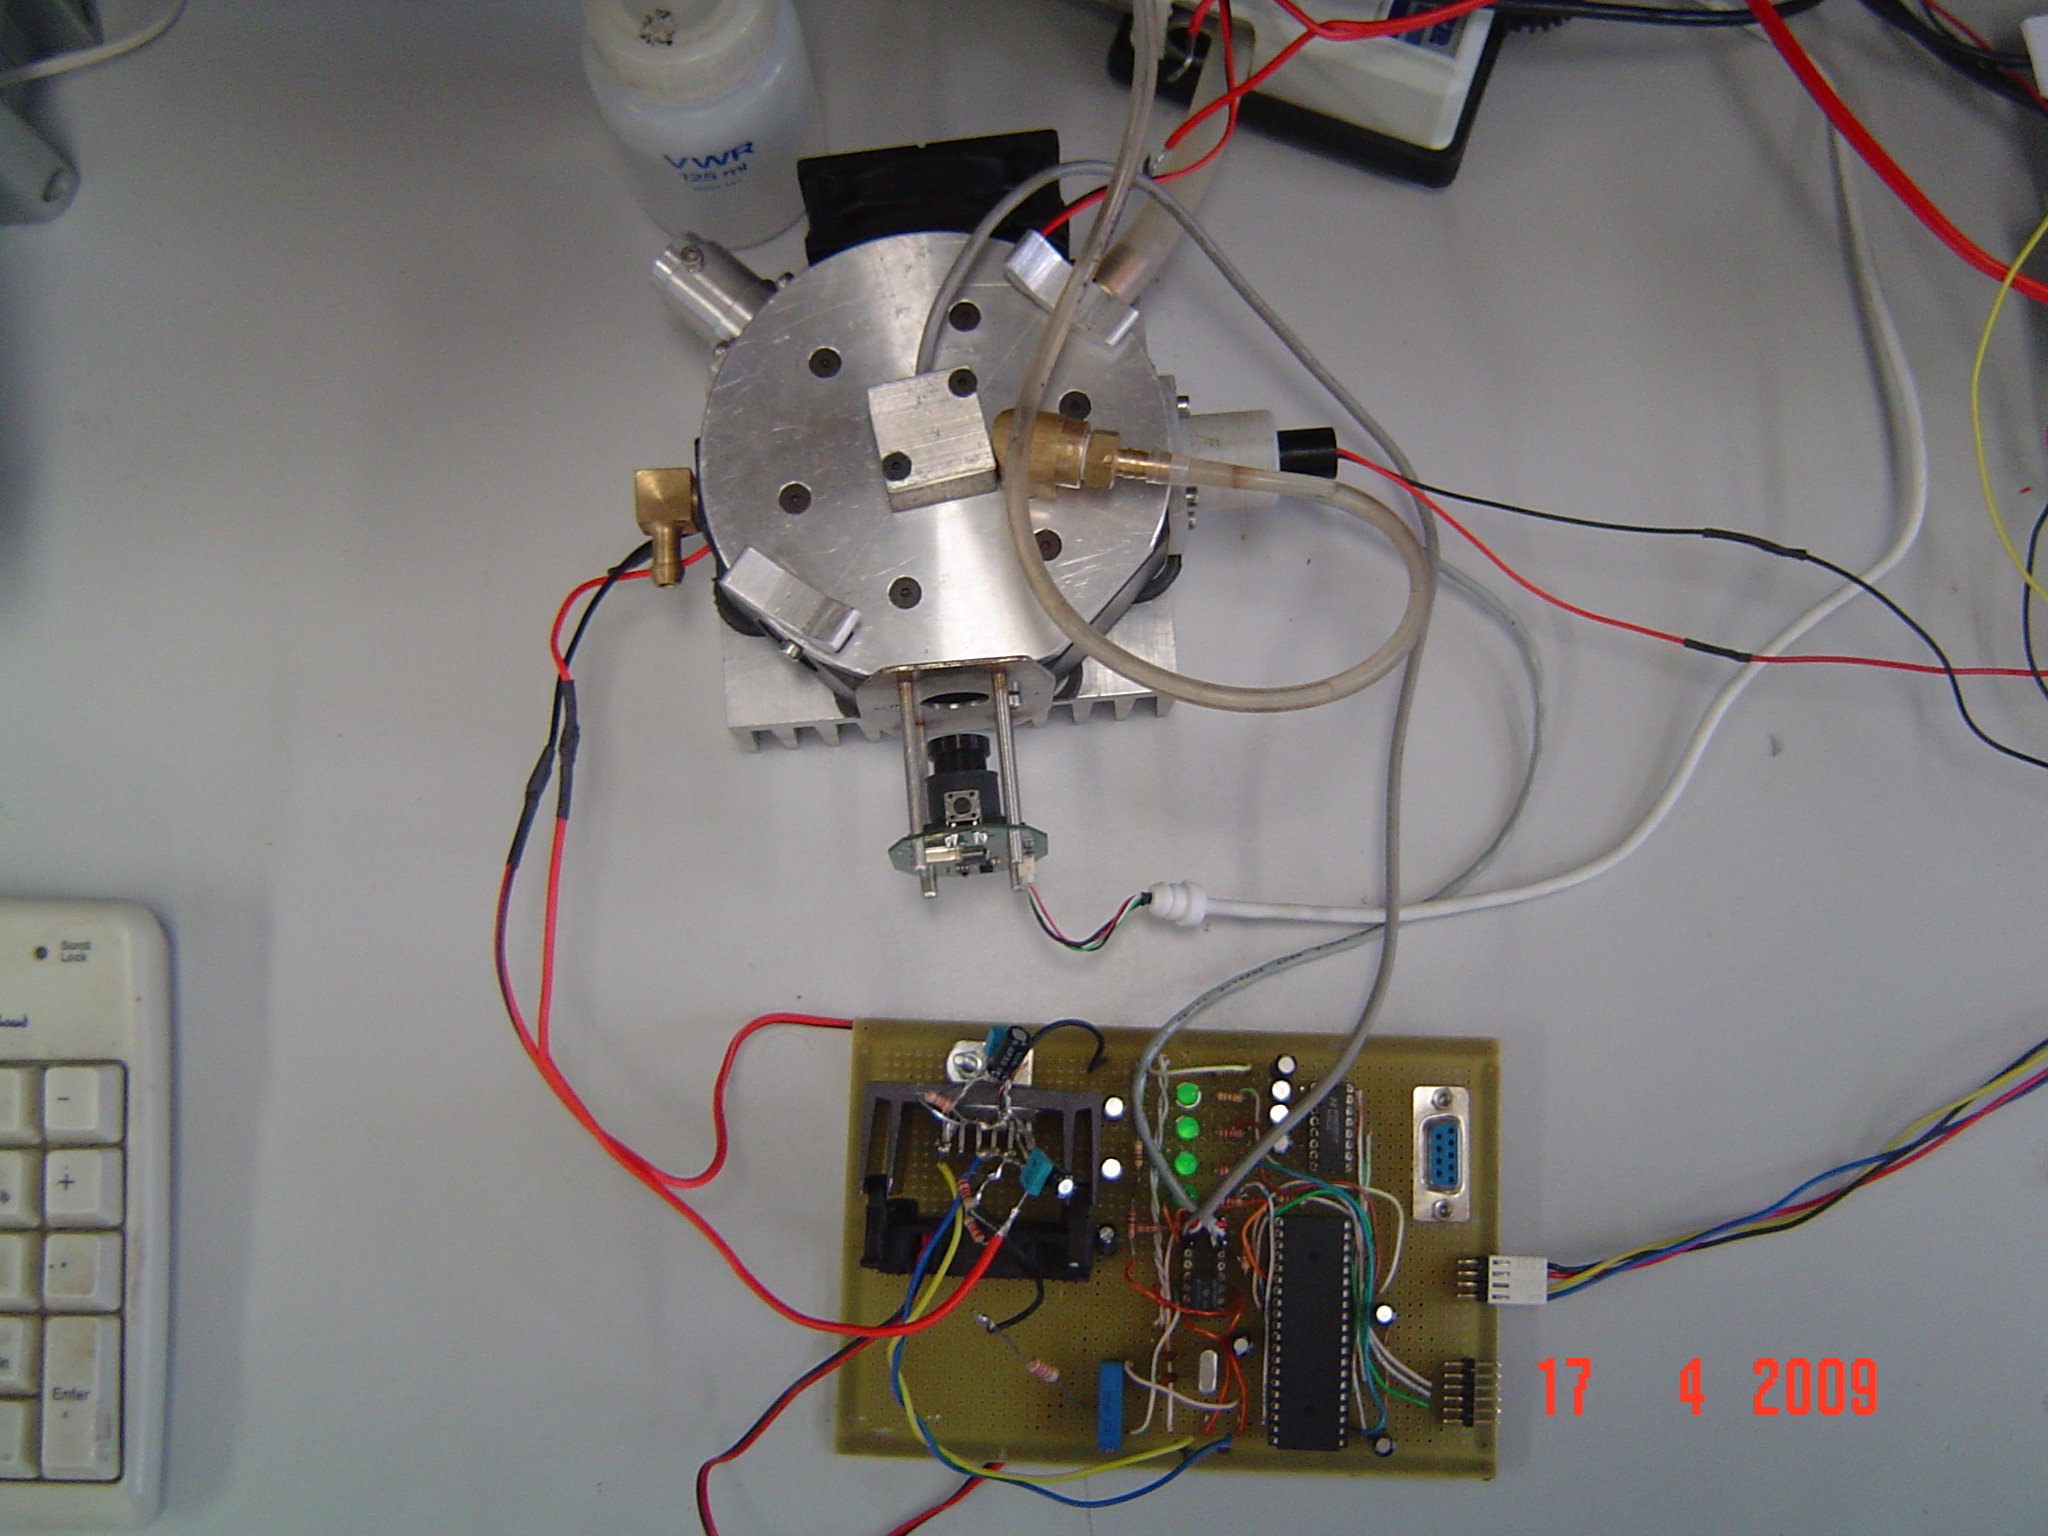
\includegraphics[scale=0.1]{eps/ccnc_detalhes_6.eps}}\\
\centering \caption{\label{6figs} detalhes da c\^{a}mara do CCNC-SDCC.}
\end{figure}


\section{Controle da Supersatura\c{c}\~{a}o}

Como reportado anteriormente, a supersatura\c{c}\~{a}o (o excesso de vapor) dentro da c\^{a}mara de nuvens \'{e} obtida atrav\'{e}s da manuten\c{c}\~{a}o de umidade nas suas tampas inferior e superior, garantida por um reservat\'{o}rio de \'{a}gua externo \`{a} c\^{a}mara, e da manuten\c{c}\~{a}o de uma diferen\c{c}a de temperatura entre as tampas inferior e superior da c\^{a}mara.


A diferen\c{c}a de temperatura entre as tampas  \'{e} mantida atrav\'{e}s do acionamento de um dispositivo termo-el\'{e}trico (tamb\'{e}m conhecido como pastilha Peltier), instalado na tampa inferior da c\^{a}mara de nuvens. Nesse caso, s\~{a}o utilizadas duas pastilhas Peltier modelo DV-30-10 fabricados pela DANVIC. Quanto \`{a} tampa superior, esta somente possui um sensor de temperatura, sendo portanto, a sua temperatura a mesma do meio ambiente.

A medida da diferen\c{c}a de temperatura entre as tampas \'{e} realizada por dois sensores iguais fixados no centro das tampas inferior e superior da c\^{a}mara de nuvens. Este  sensor \'{e} o DS18B20-PAR fabricado pela Dallas Semiconductor e fornece o valor da temperatura na forma digital com 12 bits, com uma resolu\c{c}\~{a}o de 0,0625$^o$C e com uma acur\'{a}cia de 0,5$^o$C. O valor da acur\'{a}cia, garantida pelo fabricante \'{e}, em princ\'{\i}pio, um fator restritivo ao seu uso, pois, segundo Frank et al \cite{Frank} \'{e} necess\'{a}rio uma acur\'{a}cia na medi\c{c}\~{a}o da diferen\c{c}a de temperatura de no m\'{\i}nimo 0,1$^o$C. Entretanto, considerando-se que \'{e} a diferen\c{c}a da temperatura o principal par\^{a}metro a ser considerado, utilizou-se dois sensores id\^{e}nticos.

Com o objetivo de se selecionar os sensores a serem utilizados, um experimento  foi realizado para avaliar a dispers\~{a}o dos valores medidos. Esse experimento consistiu em monitorar as medi\c{c}\~{o}es de temperaturas por 2 horas e 27 minutos de dois sensores, instalados em uma mesma chapa de alum\'{\i}nio de 2,0 mm de espessura e com uma dist\^{a}ncia de 1,0 cm um do outro. Nesse experimento foram obtidos os resultados estat\'{\i}sticos apresentados na Tabela \ref{estatistica} a seguir.

\begin{table}[!htbp]
\centering \caption{\label{estatistica} resultados estat\'{\i}sticos para os dois sensores de temperatura DS18B20-PAR.}
\begin{tabular}{ c | c }
  \hline
  Par\^{a}metro & Valor\\
  \hline
  Diferen\c{c}a m\'{e}dia & 0,0082\\
  Diferen\c{c}a m\'{\i}nima & -0,0625\\
  Diferen\c{c}a m\'{a}xima & 0,0625\\
  Desvio padr\~{a}o & 0,03\\
  N\'{u}mero de medi\c{c}\~{o}es & 8824\\
  \hline
\end{tabular}\\
\end{table}


O principal resultado apresentado na Tabela \ref{estatistica} s\~{a}o as diferen\c{c}as de temperatura m\'{a}xima e m\'{\i}nima entre os sensores, cujo valor obtido \'{e} 0,0625 $^{o}$C. Essa diferen\c{c}a garante medidas de diferen\c{c}a de temperatura abaixo de 0,1$^{o}$C necess\'{a}rios a um bom desempenho do CCNC-SDCC conforme \'{e} dito por Frank at all \cite{Frank}. Simula\c{c}\~{o}es realizadas segundo as equa\c{c}\~{o}es \ref{eq01}, \ref{eq02}, \ref{eq03} e \ref{eq04}, considerando-se a diferen\c{c}a m\'{a}xima e absoluta medidas, mostram que o erro m\'{a}ximo no valor da supersatura\c{c}\~{a}o \'{e} menor do que 3\%.

O circuito eletr\^{o}nico, mostrado na Figura \ref{crt_SDCC}, indica como \'{e} realizado o controle da diferen\c{c}a de temperatura entre as tampas. Esse circuito consiste de um controle eletr\^{o}nico de temperatura em malha fechada que se inicia a partir da escolha de uma determinada  supersatura\c{c}\~{a}o de opera\c{c}\~{a}o da c\^{a}mara de nuvens, definida pelo operador, cujo valor \'{e} inserido atrav\'{e}s do PC. Em seguida, a partir do valor medido da temperatura da tampa superior (temperatura do meio ambiente) \'{e} calculada a temperatura da tampa inferior necess\'{a}ria para que se possa obter a supersatura\c{c}\~{a}o definida pelo operador conforme as express\~{o}es \ref{eq01} a \ref{eq04}. Ent\~{a}o, essa diferen\c{c}a \'{e}  transferida ao microcontrolador (dsPIC30F4013) que, atrav\'{e}s de um sistema de controle cl\'{a}ssico do tipo PID (Proporcional Integral Diferencial), gera um sinal do tipo PWM (\emph{Pulse With Modulation}) para um conversor D/A de 1 bit. O sinal anal\'{o}gico aciona o amplificador de pot\^{e}ncia, configurado no modo inversor que, por sua vez, aciona as pastilhas Peltier.


\begin{figure}[!hbt]
\begin{center}
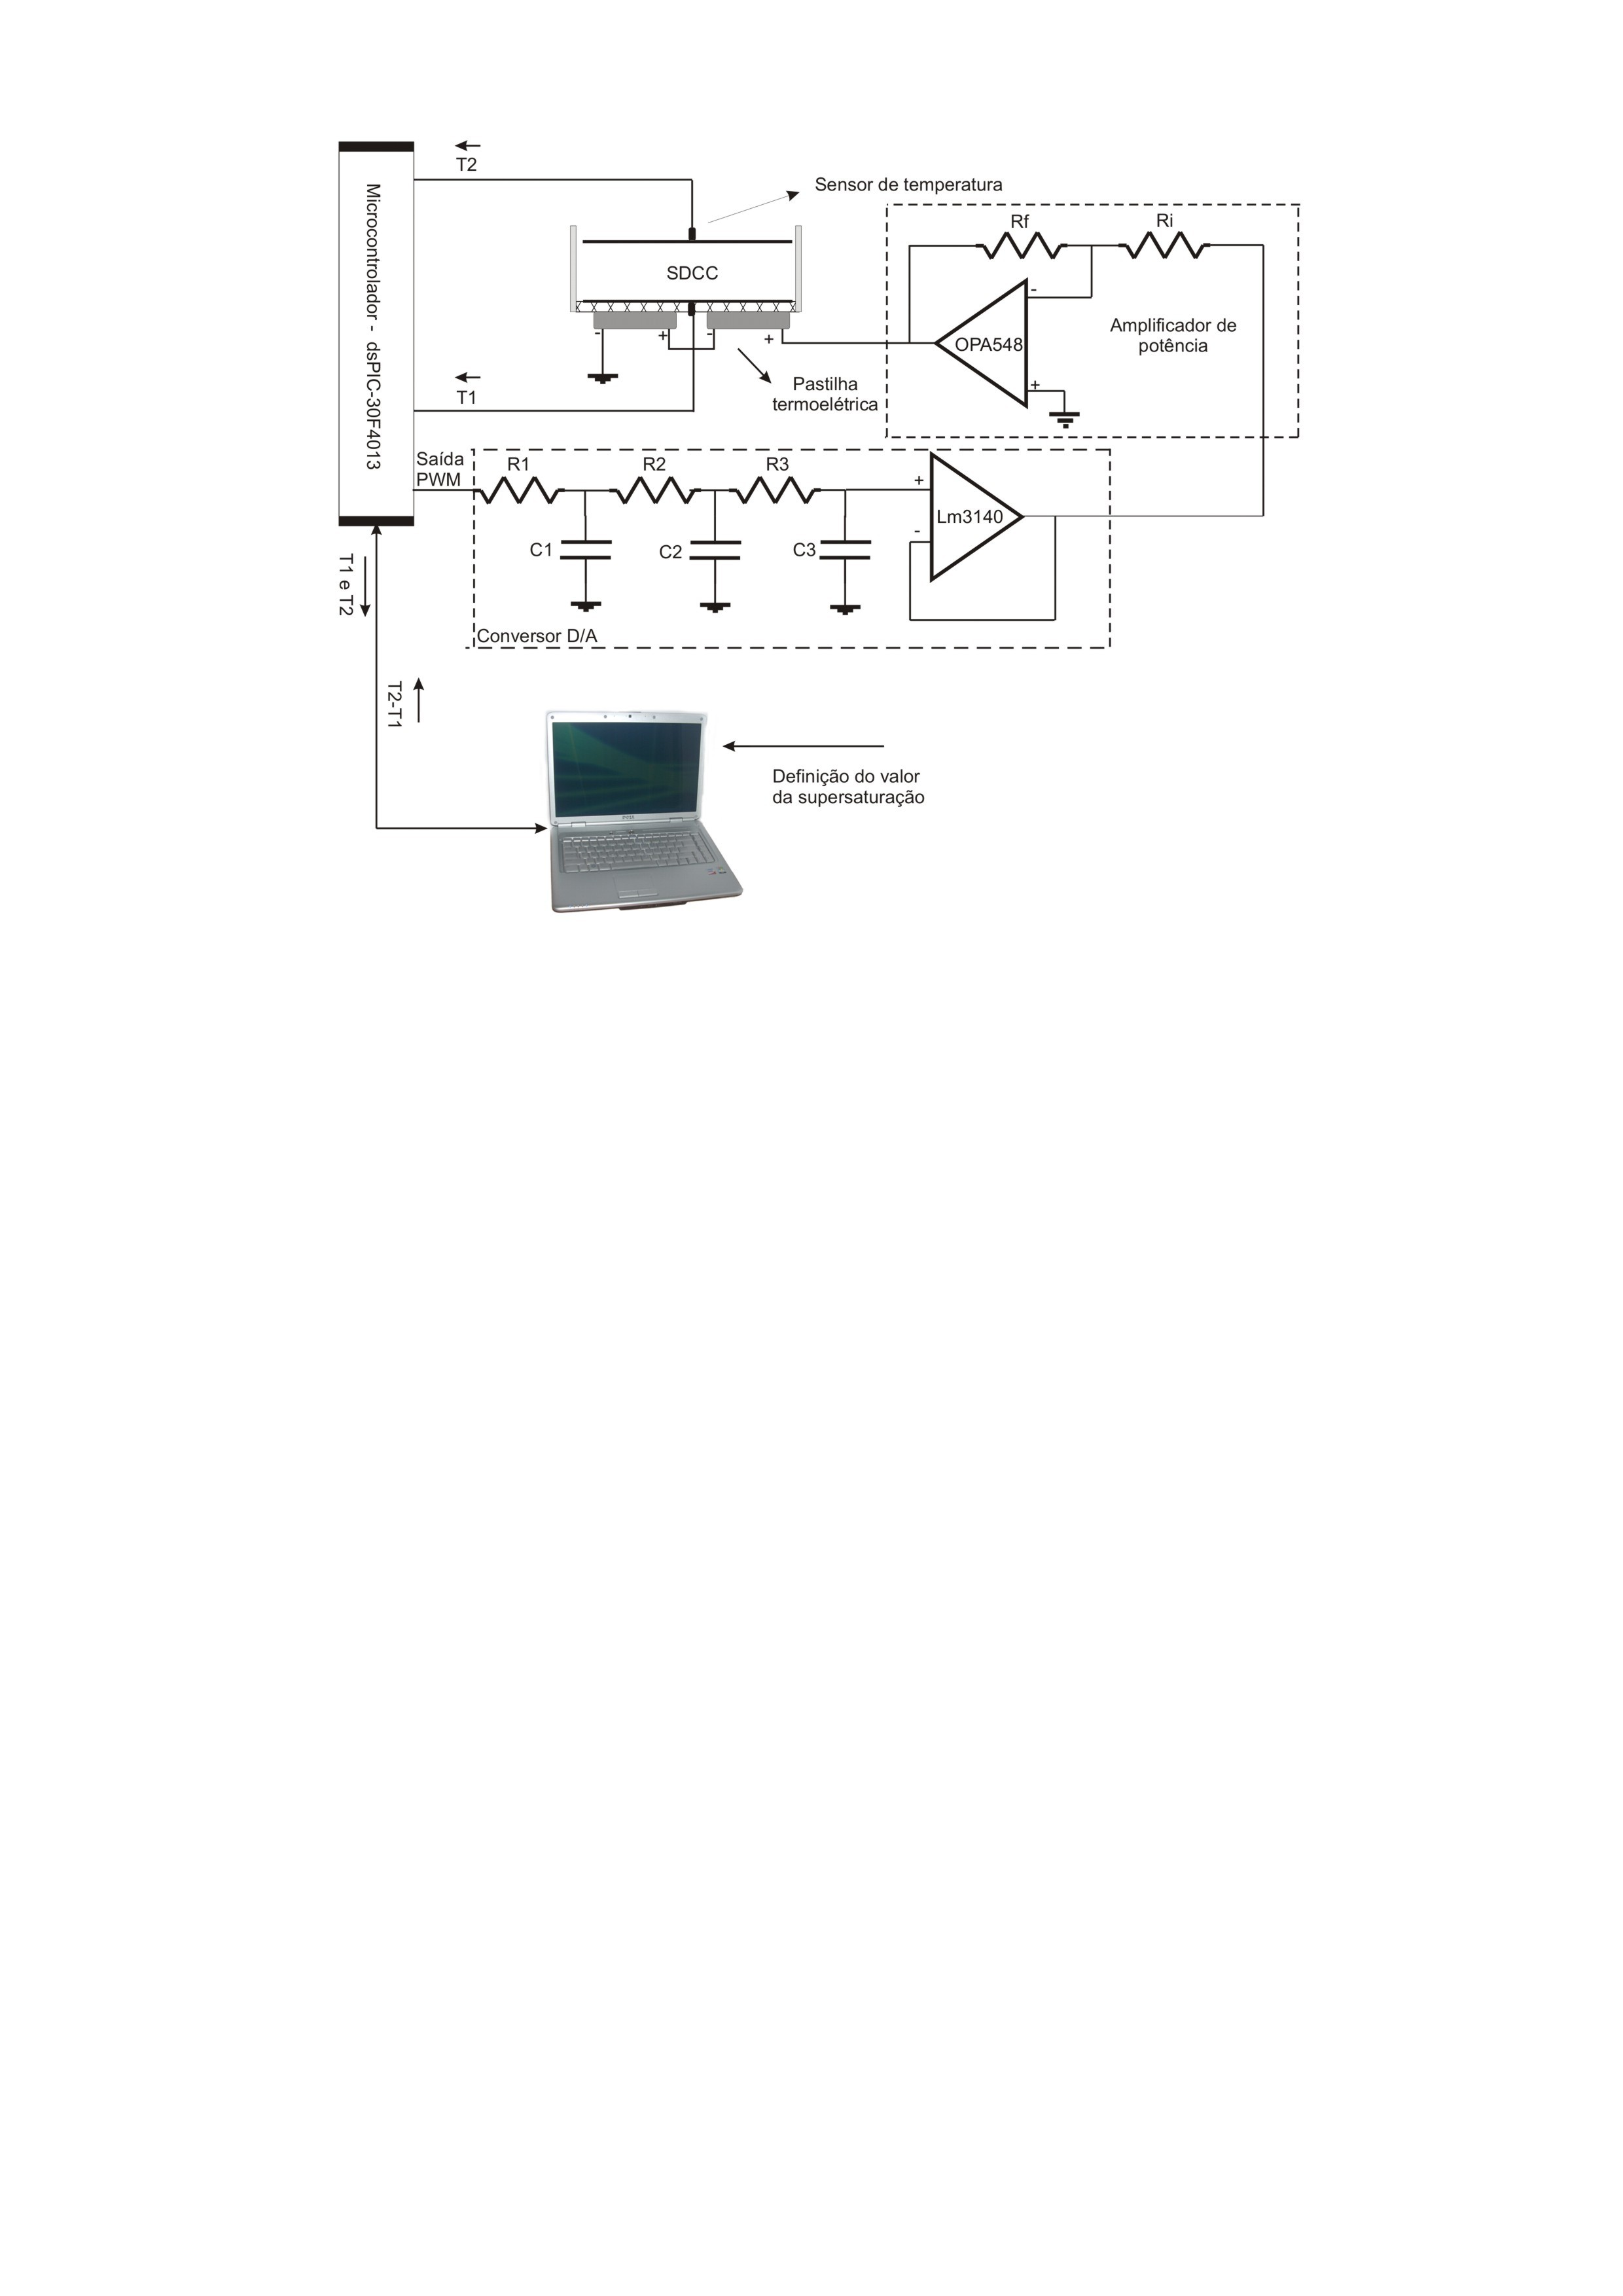
\includegraphics[scale=1.0]{eps/crt_SDCC2.eps}\\
\end{center}
\caption{\label{crt_SDCC}\hspace{-0.1em} diagrama de blocos do hardware de controle das pastilhas termo-el\'{e}tricas.}
\end{figure}

\newpage
\subsection{Unidade de controle}

A unidade de controle do CCNC-SDCC tem como n\'{u}cleo o microcontrolador dsPIC30F4013.  Esse microcoltrolador, de alto desempenho, fabricado pela Microchip, possui um arquitetura interna do tipo RISC (\emph{Reduced Instruction Set Computer}) e um \emph{chipset} que o torna capaz de realizar tanto tarefas comuns a quaisquer microcontrolador, bem como de realizar c\'{a}lculos espec\'{\i}ficos em processamento digital de sinais. Sua fun\c{c}\~{a}o \'{e} o acionamento das v\'{a}lvulas, bomba, leitura dos sensores de temperatura, gera\c{c}\~{a}o de um sinal PWM para acionamento das pastilhas Peltier a partir de um controle PID e comunica\c{c}\~{a}o com um microcomputador para interface homem-m\'{a}quina. O circuito eletr\^{o}nico completo dessa unidade de controle, cujas dimens\~{o}es s\~{a}o 15,0 cm x 10,0 cm, \'{e} mostrado no Anexo D. Esse circuito \'{e} bastante reduzido em n\'{u}mero de dispositivos eletr\^{o}nicos se comparado com o circuito de controle do CCNC-WYO que possui 5 placas eletr\^{o}nicas. Isso \'{e} poss\'{\i}vel porque todas as fun\c{c}\~{o}es do CCNC-SDCC est\~{a}o embarcadas no microcontrolador: medi\c{c}\~{a}o da temperatura, gera\c{c}\~{a}o do sinal de controle para as pastilhas termoel\'{e}tricas, acionamento da bomba, acionamento das v\'{a}lvulas e comunica\c{c}\~{a}o com computador. A \'{u}nica fun\c{c}\~{a}o que \'{e} realizada fora da unidade de controle \'{e} o processamento da imagem que \'{e} feita por um microcomputador.

%\newpage
%\begin{figure}[!hbt]
%    \begin{center}
%        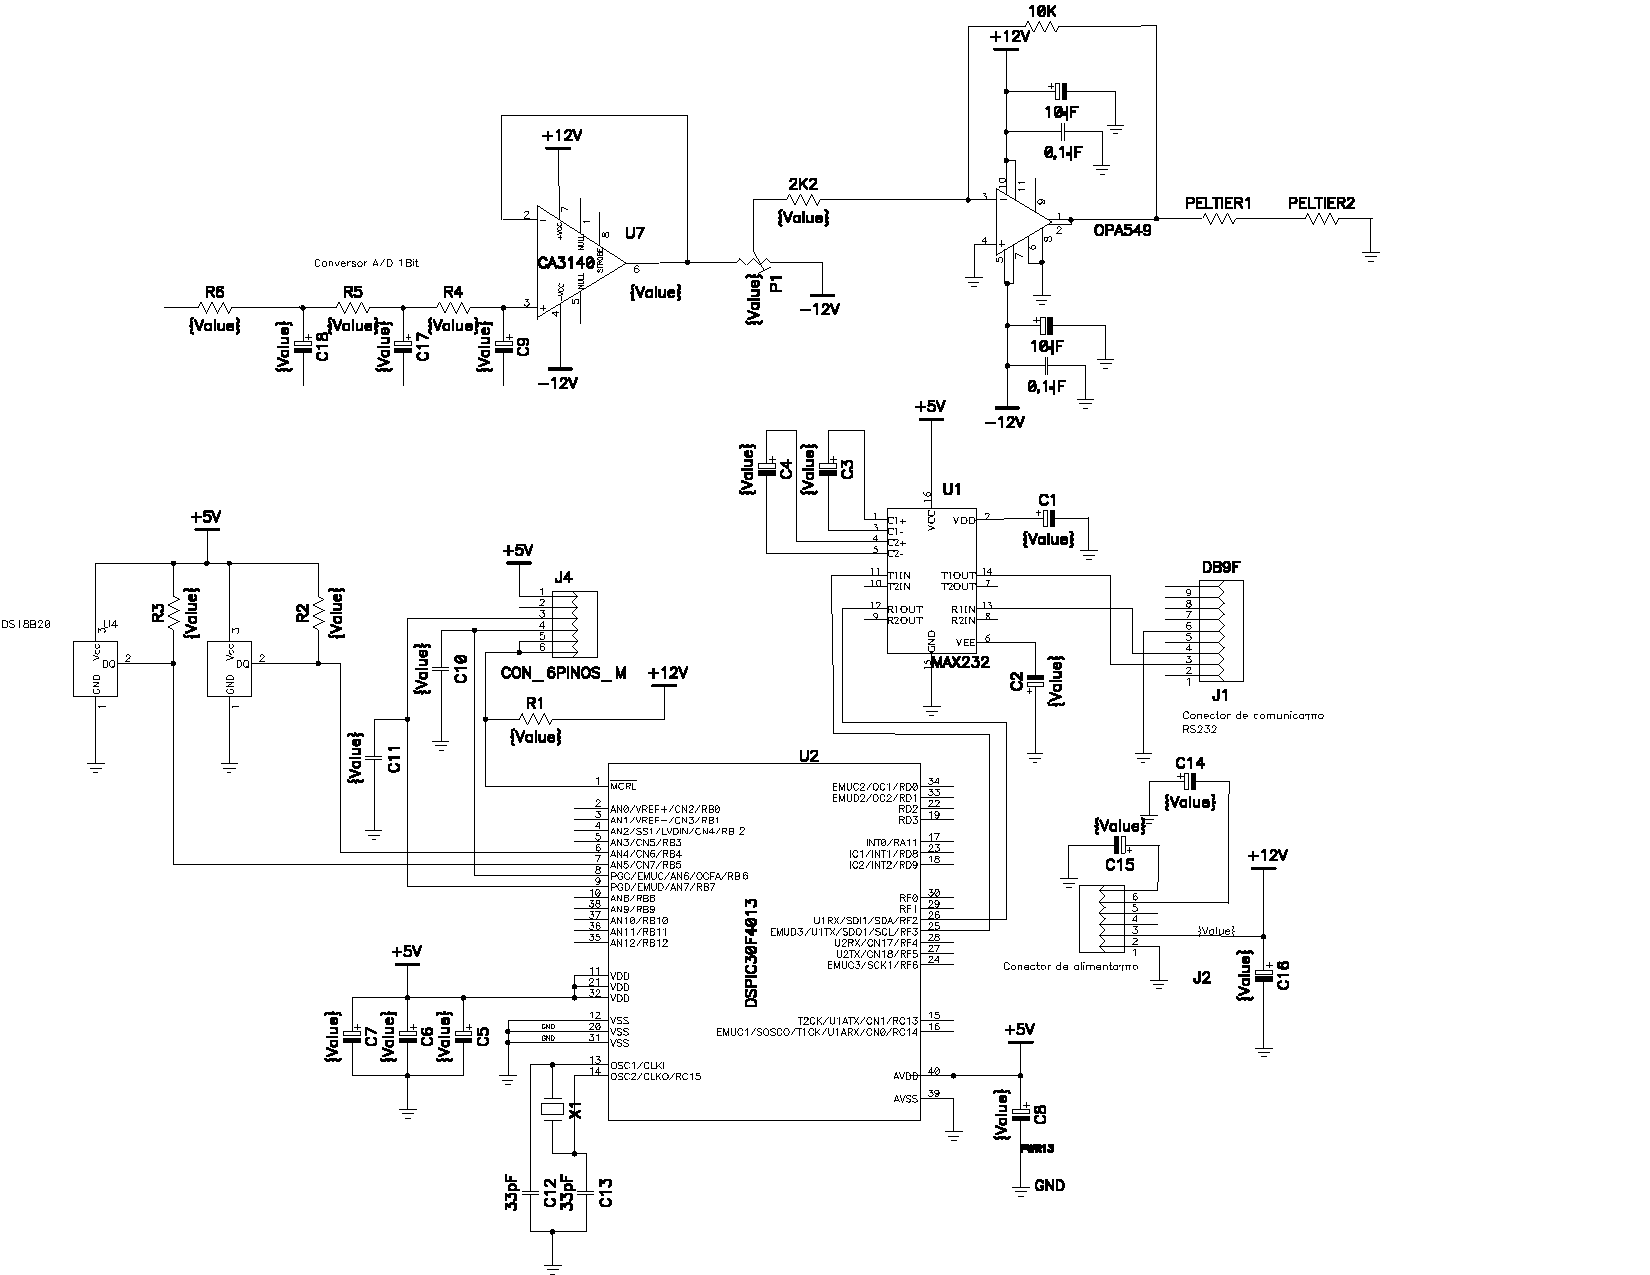
\includegraphics[bb=1.0in 12.0in 7.5in 10in,scale=0.9]{eps/ccncsch.pdf}
%    \end{center}
%    \caption{\label{ccncsch}\hspace{-0.1em} diagrama el\'{e}trico da unidade de controle do CCNC-SDCC.}
%\end{figure}
%\newpage


\subsection{Software CCNC-SDCC ver1.0}

O software CCNC-SDCC (vers\~{a}o 1.0) consiste de um programa computacional com dois n\'{u}cleos importantes e \'{e} executado em um computador pessoal com sistema operacional \emph{Windows}. O primeiro n\'{u}cleo permite a intera\c{c}\~{a}o entre o operador e a unidade de controle do CCNC-SDCC. Trata-se, portanto, de uma interface homem-m\'{a}quina. O segundo n\'{u}cleo processa a imagem, em tempo real, e informa o n\'{u}mero de got\'{\i}culas dentro do volume de amostragem e, consequentemente, calcula a concentra\c{c}\~{a}o dessas got\'{\i}culas e, portanto, a concentra\c{c}\~{a}o de aeross\'{o}is.

O n\'{u}cleo respons\'{a}vel pela interface homem-m\'{a}quina foi constru\'{\i}do utilizando-se o sistema de desenvolvimento C++ Builder vers\~{a}o 6.0. Foram criadas tr\^{e}s telas de interface. A primeira, que \'{e} apresentada da Figura \ref{CCNCTELA01}, \'{e} a principal. Essa tela permite as seguintes a\c{c}\~{o}es: a sele\c{c}\~{a}o de quais supersatura\c{c}\~{o}es que devem ser induzidas no interior da c\^{a}mara, o disparo do ciclo de medi\c{c}\~{a}o e a visualiza\c{c}\~{a}o de gotas. Al\'{e}m disso, apresenta as temperaturas inferior e superior, a diferen\c{c}a de temperatura entre as tampas, n\'{u}mero de gotas e, por fim, o valor obtido da concentra\c{c}\~{a}o dos n\'{u}cleos de condensa\c{c}\~{a}o de nuvens.

\begin{figure}[!hbt]
\begin{center}
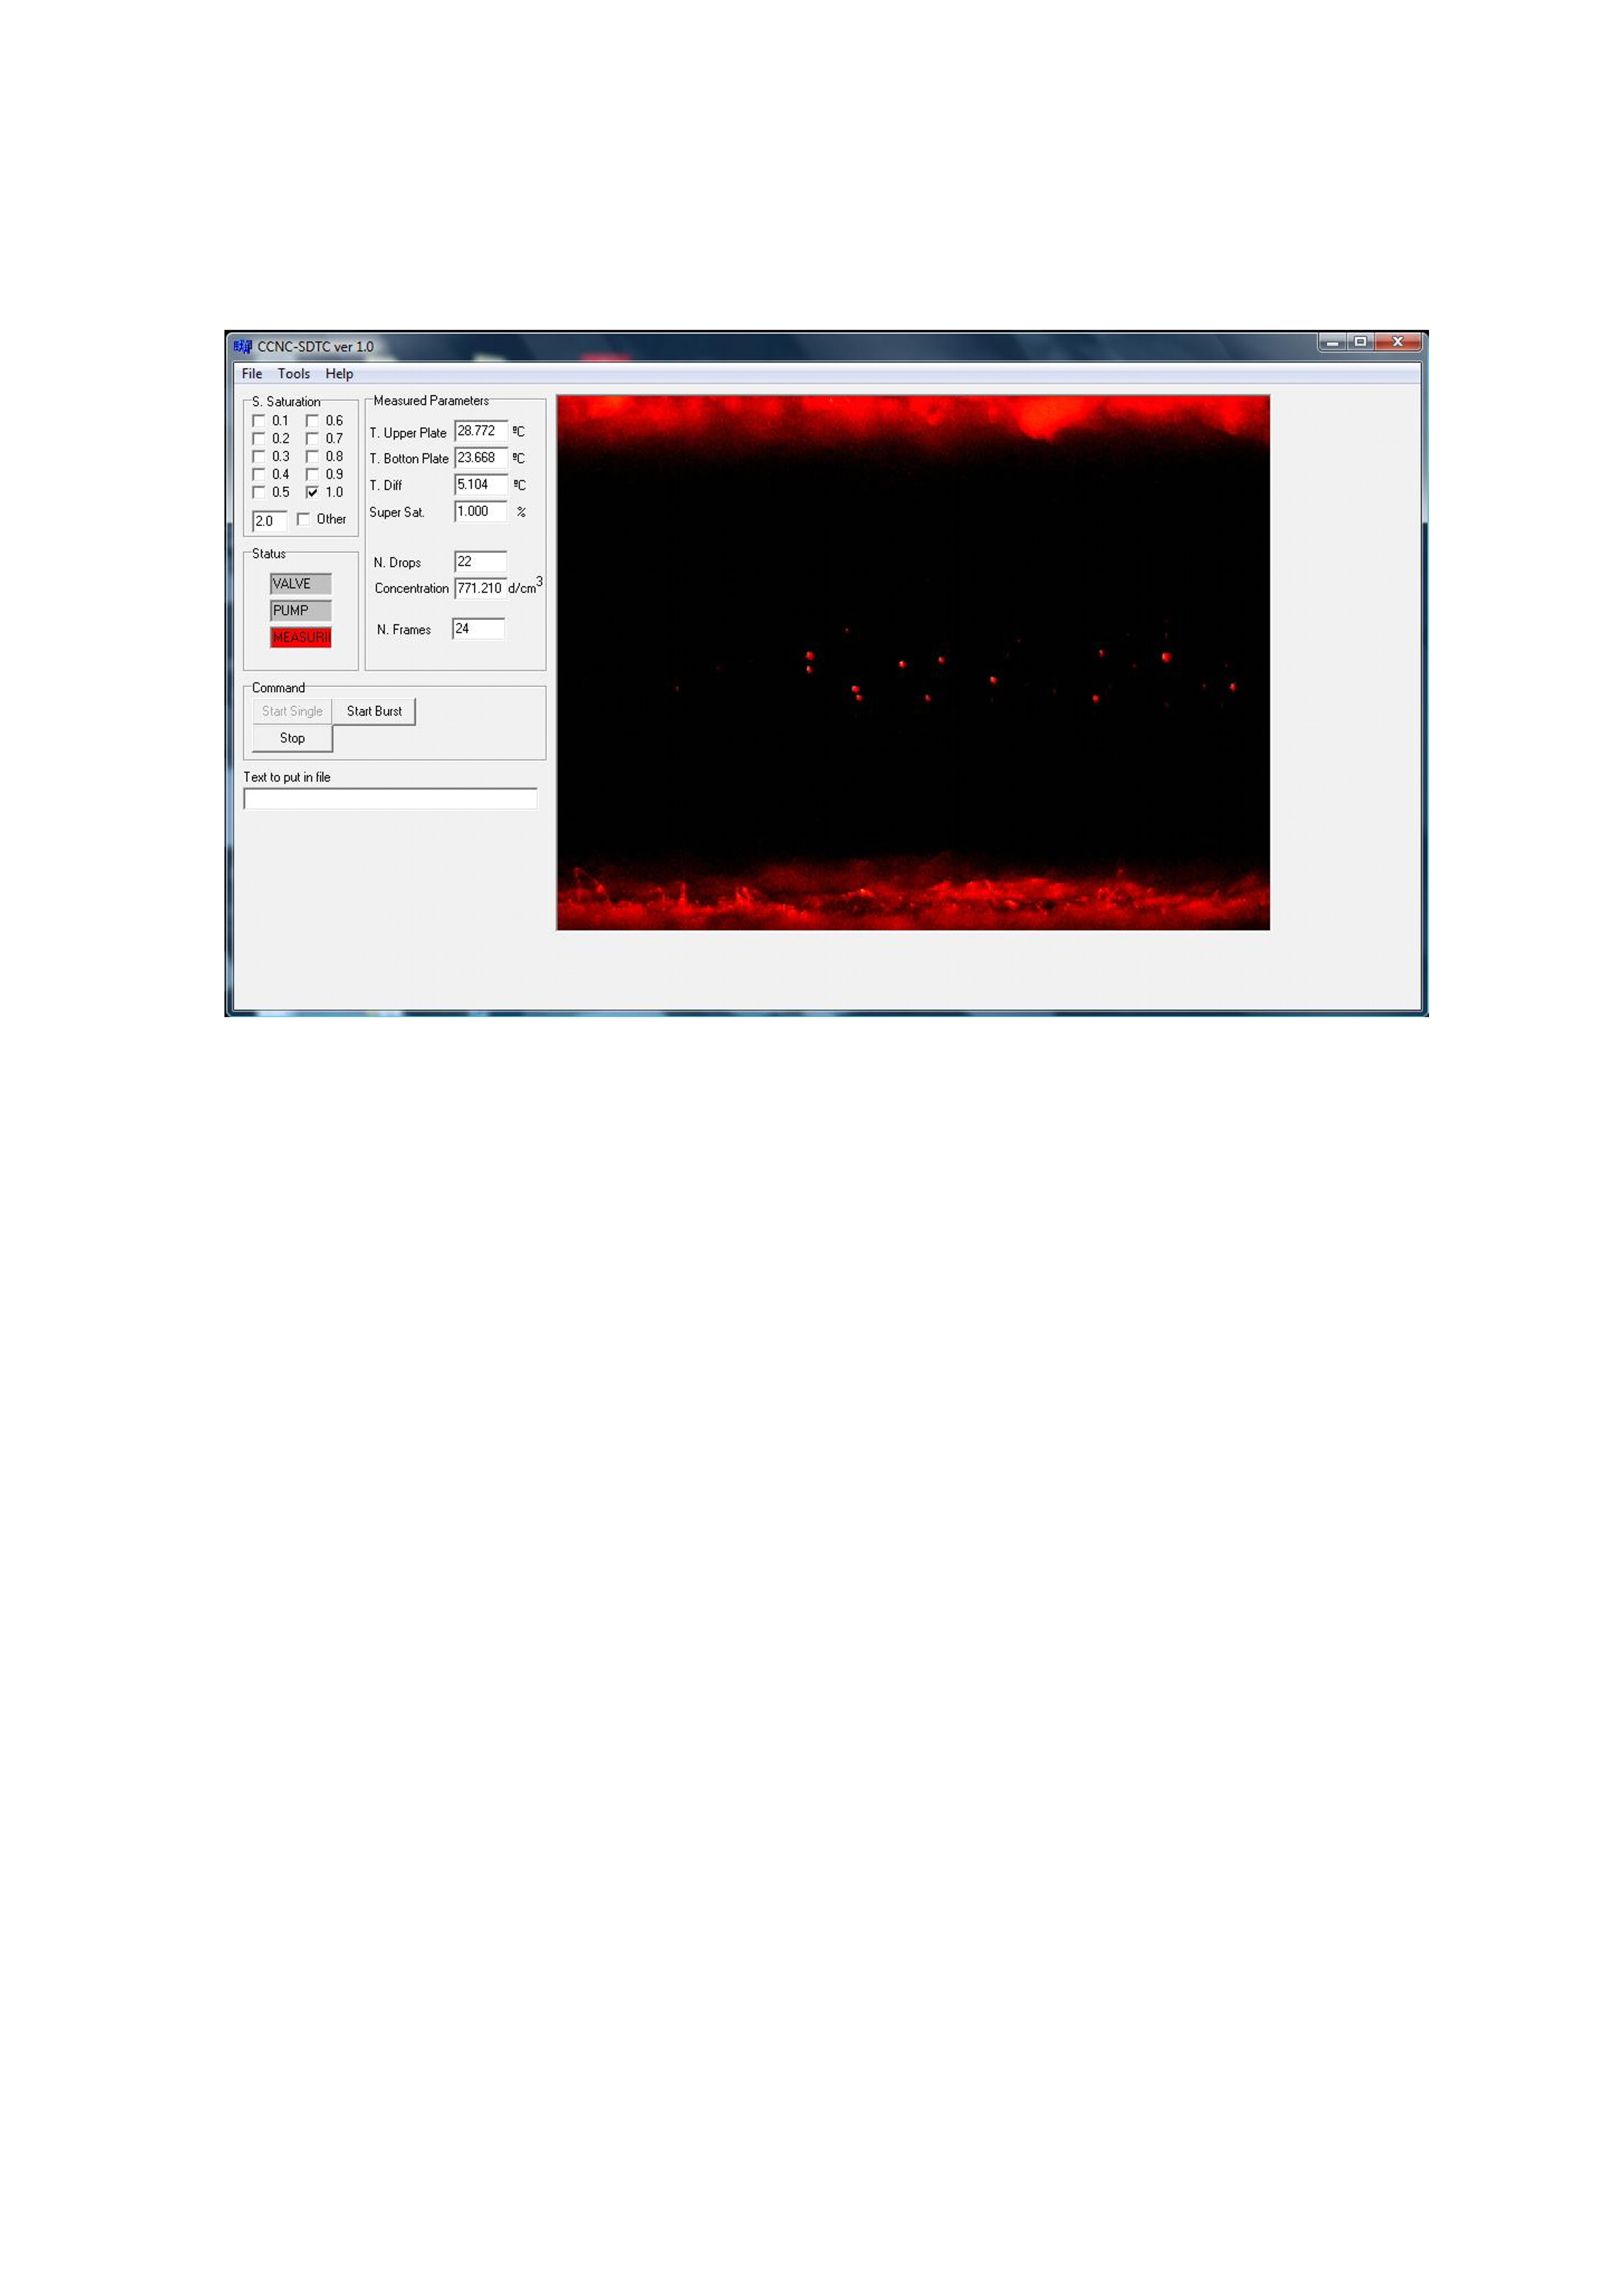
\includegraphics[scale=0.8]{eps/CCNCTELA01.eps}\\
\end{center}
\caption{\label{CCNCTELA01}\hspace{-0.1em} tela principal do CCNC-SDCC.}
\end{figure}

 As duas telas seguintes s\~{a}o telas de servi\c{c}o e de configura\c{c}\~{a}o operacional. A tela de servi\c{c}o, mostrada na Figura \ref{CCNC_TELA03}, permite o acionamento ass\'{\i}ncrono da bomba, das v\'{a}lvulas, das pastilhas Peltier e a visualiza\c{c}\~{a}o das imagens no interior da c\^{a}mara de nuvens. A tela de configura\c{c}\~{a}o operacional, mostrada na Figura \ref{CCNC_TELA02}, permite o ajuste do volume de amostragem, do n\'{\i}vel de ilumina\c{c}\~{a}o da c\^{a}mara, do n\'{\i}vel de limiar de detec\c{c}\~{a}o e do per\'{\i}odo de medi\c{c}\~{a}o. Isso \'{e} feito digitando-se os valores de configura\c{c}\~{a}o nos campos existentes e, em seguida acionando-se o bot\~{a}o \emph{SAVE}.


 \begin{figure}[!hbt]
\begin{center}
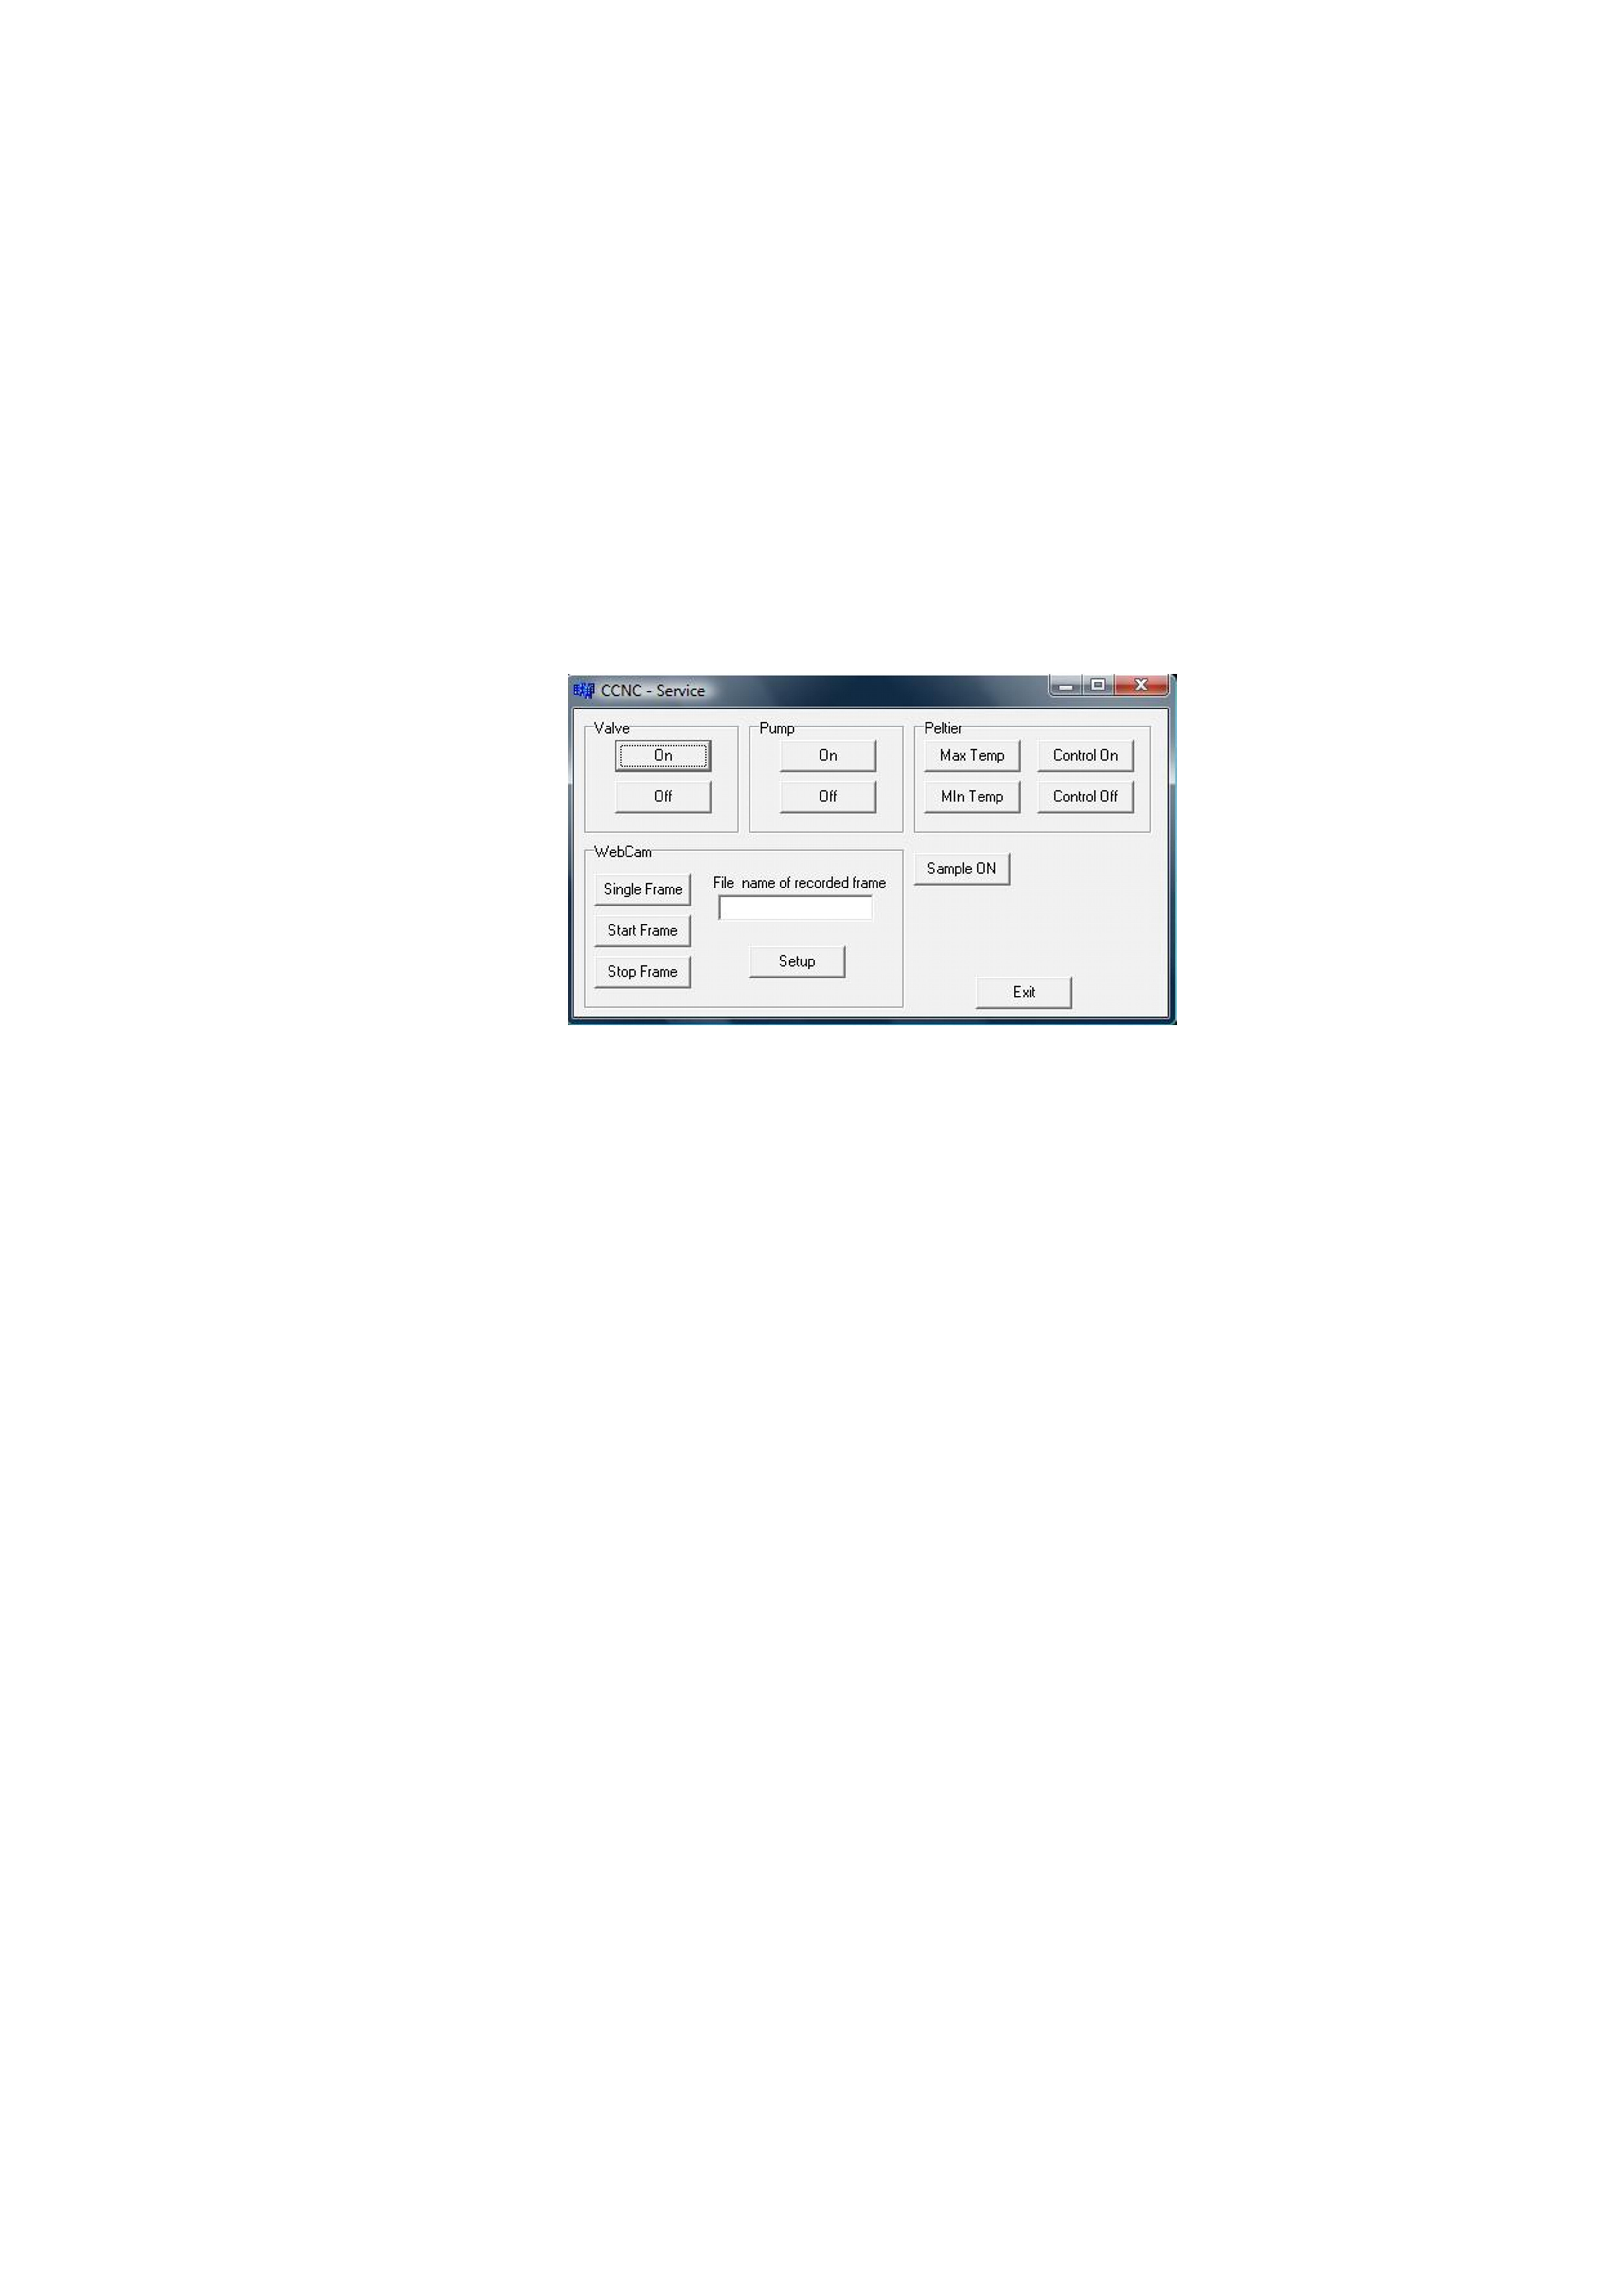
\includegraphics[scale=0.8]{eps/CCNCtela03.eps}\\
\end{center}
\caption{\label{CCNC_TELA03}\hspace{-0.1em} tela de servi\c{c}o.}
\end{figure}


\begin{figure}[!hbt]
\begin{center}
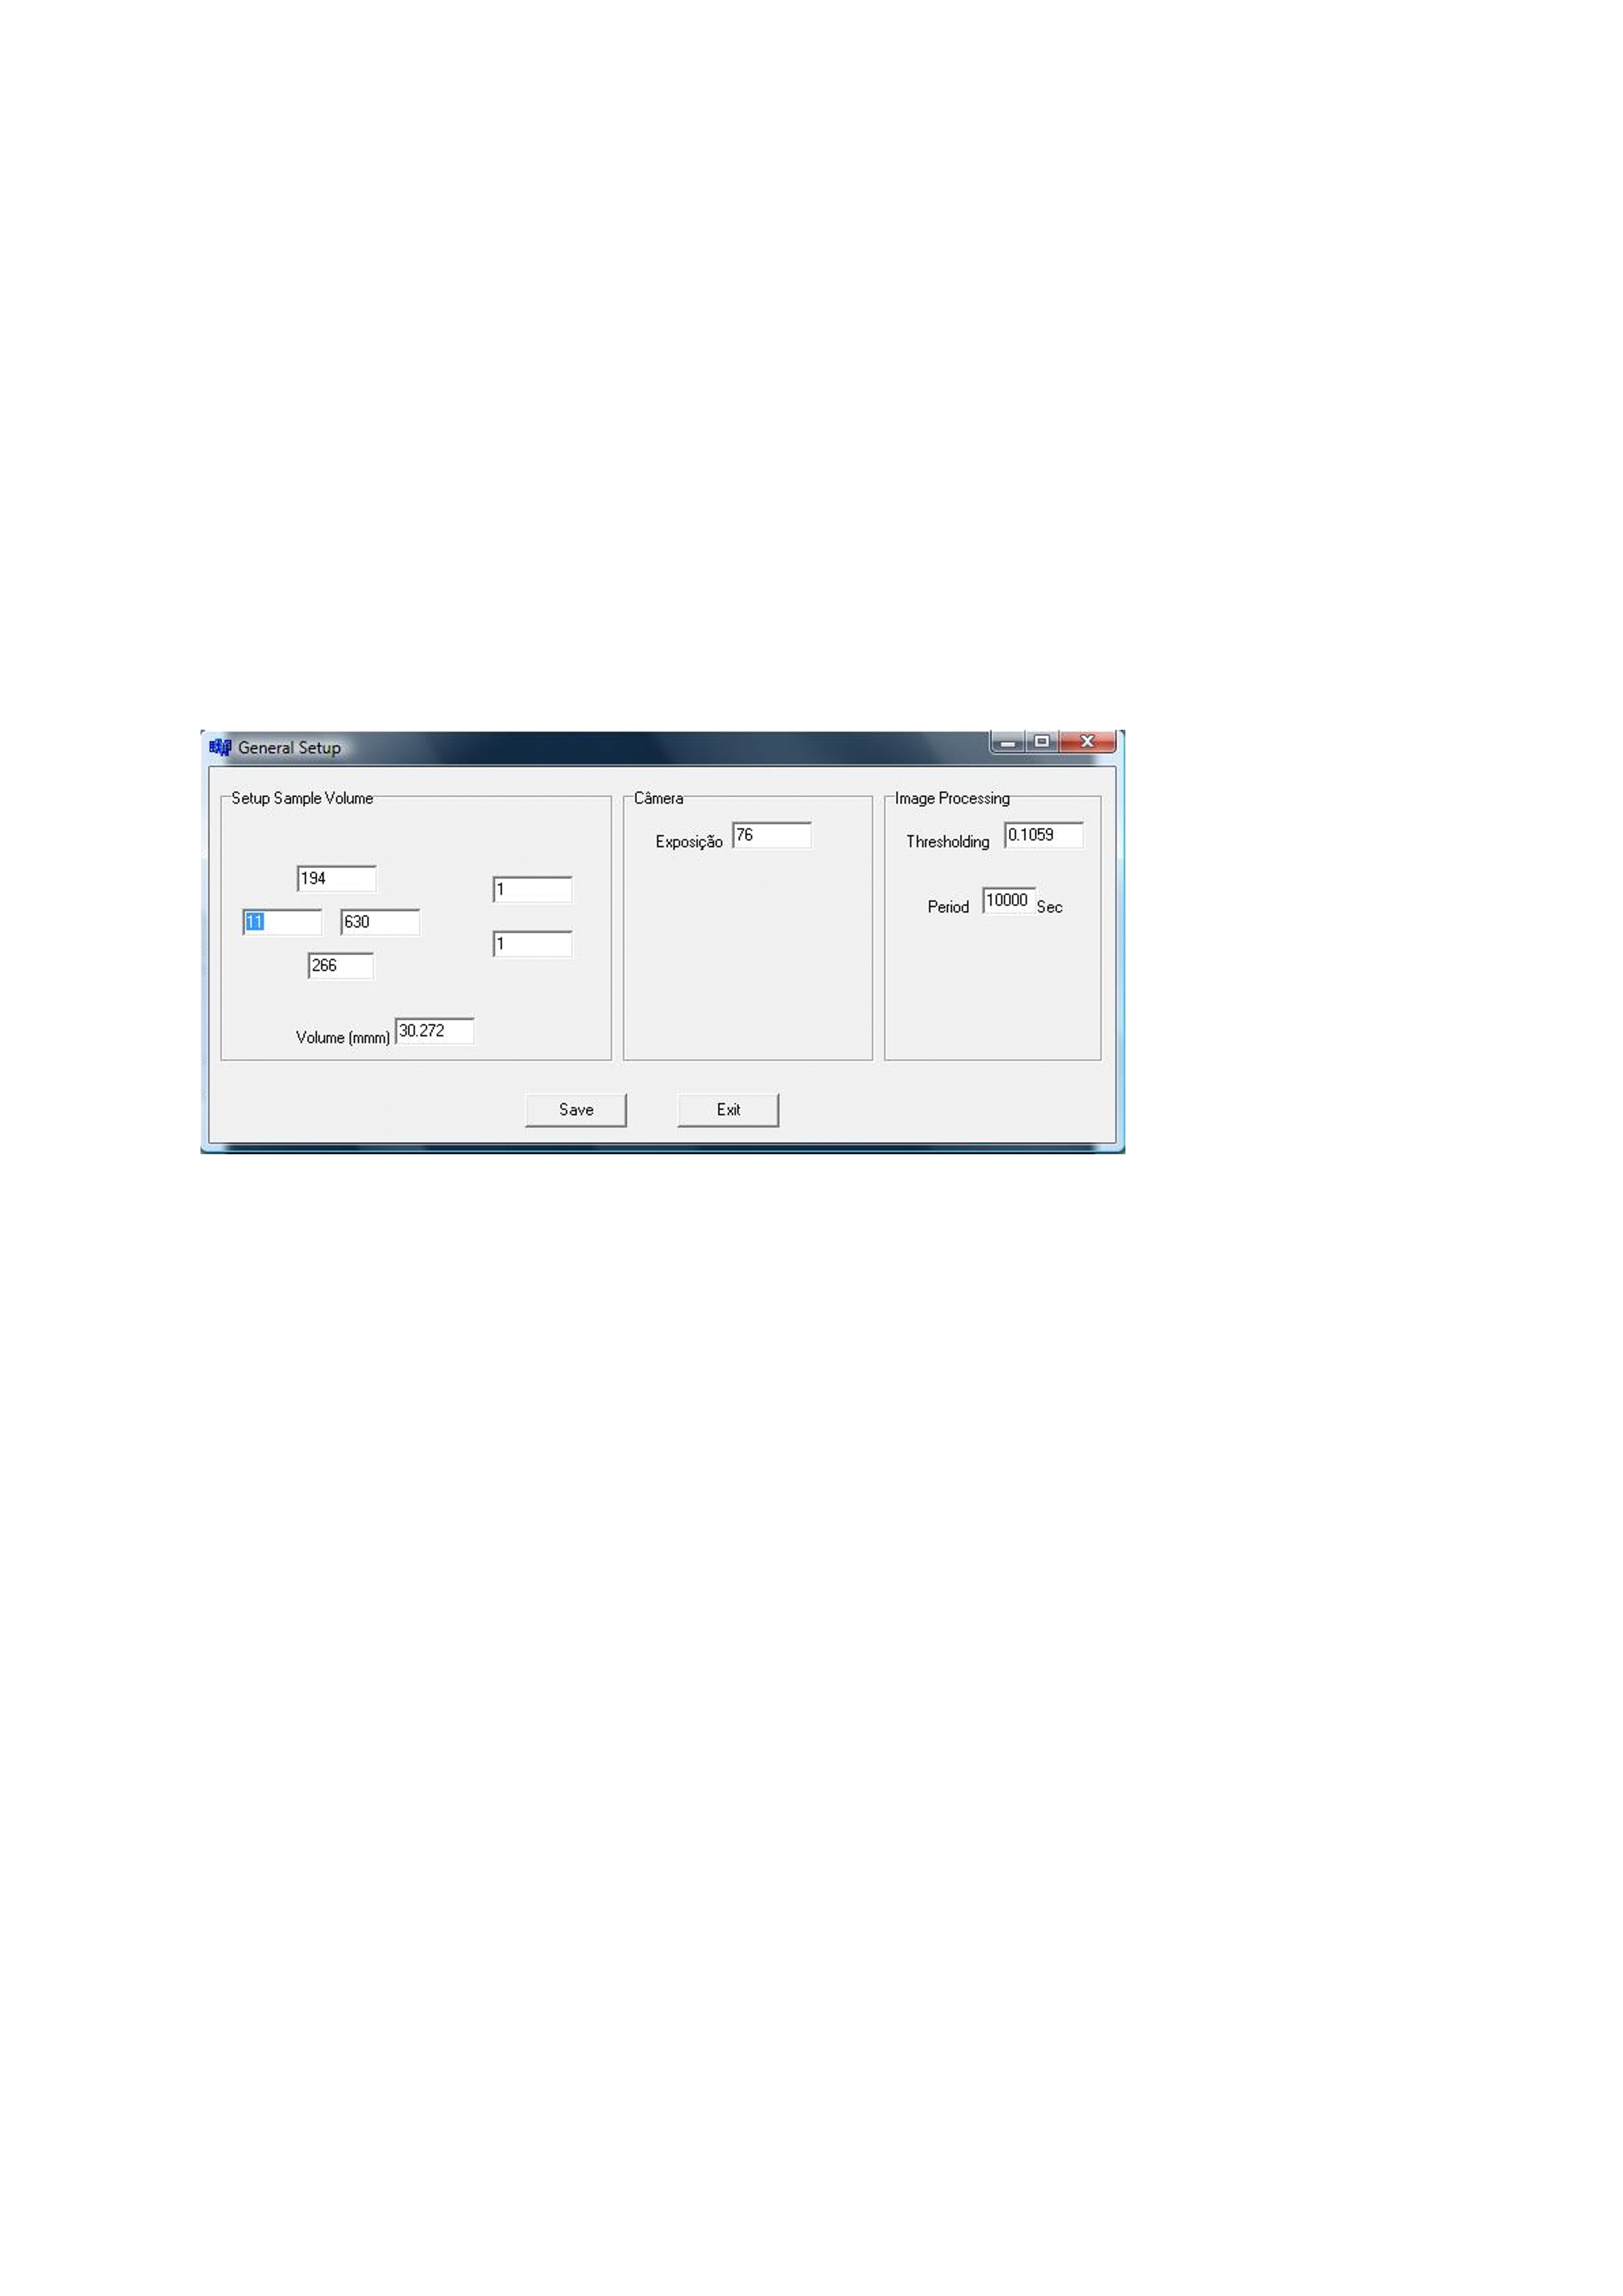
\includegraphics[scale=0.8]{eps/CCNCtela02.eps}\\
\end{center}
\caption{\label{CCNC_TELA02}\hspace{-0.1em} tela de configura\c{c}\~{a}o operacional.}
\end{figure}



O n\'{u}cleo de vis\~{a}o computacional foi desenvolvido inteiramente obedecendo o padr\~{a}o ANSI da linguagem de programa\c{c}\~{a}o C. Isto permite que este n\'{u}cleo seja facilmente transportado para outro ambiente computacional.


\section{Descri\c{c}\~{a}o dos algoritmos usados no CCNC-SDCC proposto}
Como mencionado anteriormente o n\'{u}mero de part\'{\i}culas ativadas na c\^{a}mara de nuvens pode ser obtido de forma indireta, atrav\'{e}s da medi\c{c}\~{a}o da intensidade de luz espalhada pela got\'{\i}cula de \'{a}gua ao cruzar um feixe de luz, ou direta pela contagem das got\'{\i}culas atrav\'{e}s das t\'{e}cnicas de vis\~{a}o computacional. A t\'{e}cnica indireta apresenta diversos fatores que comprometem significativamente a sua acur\'{a}cia, como por exemplo o fato da intensidade de luz espalhada ser dependente do tamanho da got\'{\i}cula de \'{a}gua. Entretanto, o mesmo n\~{a}o ocorre com a t\'{e}cnica de contagem direta por vis\~{a}o computacional cuja principal caracter\'{\i}stica \'{e} o fato de ser independente do tamanho da got\'{\i}cula. A limita\c{c}\~{a}o nessa t\'{e}cnica, ao menos at\'{e} o presente momento, consiste em medir alta concentra\c{c}\~{a}o onde o n\'{u}mero de got\'{\i}culas sobrepostas na imagem \'{e} grande. Entretanto, com a combina\c{c}\~{a}o de t\'{e}cnicas de processamento de sinais \'{e} poss\'{\i}vel aumentar significativamente a capacidade de medi\c{c}\~{a}o em altas concentra\c{c}\~{o}es.

A segmenta\c{c}\~{a}o de objetos sobrepostos em imagens tem sido bastante estudada, uma vez que este \'{e} um problema cuja solu\c{c}\~{a}o robusta \'{e} fundamental em v\'{a}rios processos de automa\c{c}\~{a}o \cite{Schmitt,Albuquerque,Pavlidis,Felix,Norberto}. O m\'{e}todo da transformada \emph{watershed} tem sido utilizado em diversas aplica\c{c}\~{o}es onde o problema da segmenta\c{c}\~{a}o de objetos sobrepostos est\'{a} presente nas imagens \cite{Xiaodong,Mao,Parvati,Li,Xie}.

A seguir s\~{a}o postos os principais conceitos em processamento de imagens aplicados ao CCNC-SDCC.


\subsection{Conceitos b\'{a}sicos de processamento digital de imagens}
O elemento b\'{a}sico de uma imagem digital \'{e} o \textit{pixel} (\textit{picture element}). Este representa uma intensidade radiom\'{e}trica dentro de uma escala que, dependendo do elemento sensor de imagem, varia por exemplo  de 0 (preto) a 255 (branco) nas imagens representadas em n\'{\i}veis de cinza. Outro par\^{a}metro importante na defini\c{c}\~{a}o de um \textit{pixel} \'{e} a sua localiza\c{c}\~{a}o no plano. Assim sendo, uma imagem digital consiste de uma fun\c{c}\~{a}o \textit{f}(\textit{x,y}), em que \textit{x} e \textit{y} s\~{a}o as coordenadas de um valor de intensidade radiom\'{e}trica. A partir dessa defini\c{c}\~{a}o de imagem digital diversas opera\c{c}\~{o}es matem\'{a}ticas podem ser perfeitamente aplicadas, podendo resultar na melhoria de contraste, identifica\c{c}\~{a}o de descontinuidades, equaliza\c{c}\~{a}o de histogramas entre outros atributos \cite{Gonzales}.

Em uma imagem digital, a vizinhan\c{c}a de um \textit{pixel} \'{e} importante na defini\c{c}\~{a}o de v\'{a}rias propriedades e conceitos, dentre outros o conceito de regi\~{a}o conectada. Considerando-se uma imagem digital como sendo uma grade retangular, um conjunto de \textit{pixels} pode ser, em rela\c{c}\~{a}o a um \textit{pixel} central e adjacente, um vizinho tipo 4 ou tipo 8. Chama-se vizinhan\c{c}a 4 de um \textit{pixel P}, todos os \textit{pixels} adjacentes a \textit{P}, localizados fora da diagonal que passa por \textit{P}, e de vizinhan\c{c}a 8 de um \textit{pixel P} todos os \textit{pixels} que s\~{a}o adjacentes a \textit{P}. Nos dois casos, ainda \'{e} necess\'{a}rio que os \textit{pixels} obede\c{c}am a algum crit\'{e}rio de similaridade referente a seus n\'{\i}veis de intensidade e ou cor. Assim sendo, uma regi\~{a}o (objeto) \'{e} dita conectada quando todos os seus \textit{pixels} s\~{a}o adjacentes segundo a vizinhan\c{c}a 4 ou vizinhan\c{c}a 8. Na Figura \ref {conectado} (a) \'{e} apresentada uma estrutura de vizinhan\c{c}a 4, na Figura \ref {conectado} (b) \'{e} apresentada uma estrutura de vizinhan\c{c}a 8 e na Figura \ref {conectado} (c) \'{e} apresentado um caso que, dependendo do tipo de vizinhan\c{c}a escolhida, considera-se como sendo uma regi\~{a}o conectada, ou seja, um objeto com \textit{pixels} de vizinhan\c{c}a 8 ou duas regi\~{o}es conectadas, ou seja, dois objetos com \textit{pixels} de vizinhan\c{c}a 4 \cite{bernd}.

\begin{figure}[hbt]
\begin{center}

\includegraphics[scale=1.0]{eps/conectado1.eps}\\
\end{center}
\caption{\label{conectado}\hspace{-0.1em} exemplos de vizinhan\c{c}a tipo 4(a), tipo 8(b) e elemento conectado(c).}
\end{figure}

Como dito anteriormente, as opera\c{c}\~{o}es matem\'{a}ticas, ou transforma\c{c}\~{o}es, tamb\'{e}m s\~{a}o aplic\'{a}veis \`{a}s imagens digitais. A transforma\c{c}\~{a}o de dist\^{a}ncia, por exemplo, consiste em converter uma imagem digital bin\'{a}ria em uma outra representada em n\'{\i}veis de cinza.  Essa transforma\c{c}\~{a}o tem como base a substitui\c{c}\~{a}o de um \emph{pixel} branco da imagem bin\'{a}ria $g(x,y)$, por outro cujo valor (intensidade do n\'{\i}vel de cinza) representa a dist\^{a}ncia $d(x,y)$ deste \textit{pixel} branco a um \textit{pixel} preto ($x_i,y_i$) mais pr\'{o}ximo conforme a seguinte equa\c{c}\~{a}o:

\begin{equation}
\label{eqDist}
 d(x,y) = \min dist\{ (x,y),(x_i ,y_i )\}, \\
 (x_i ,y_i ) \in borda\ do\ objeto. \\
\end{equation}

Algumas m\'{e}tricas de dist\^{a}ncia podem ser utilizadas como por exemplo a Euclidiana, City Block e Chessboard \cite{Ricardo}. A mais comum das m\'{e}tricas \'{e} a dist\^{a}ncia Euclidiana, pois, \'{e} a mais adequada quando se busca modelar dados geom\'{e}tricos do ambiente humano. Contudo, devido a simplicidade computacional, utiliza-se nesse trabalho a m\'{e}trica Chessboard dada por:



% MathType!MTEF!2!1!+-
% feqaeaartrvr0aaatCvAUfeBSjuyZL2yd9gzLbvyNv2CaerbuLwBLn
% hiov2DGi1BTfMBaeXatLxBI9gBaebbnrfifHhDYfgasaacH8srps0l
% bbf9q8WrFfeuY-Hhbbf9v8qqaqFr0xc9pk0xbba9q8WqFfea0-yr0R
% Yxir-Jbba9q8aq0-yq-He9q8qqQ8frFve9Fve9Ff0dmeaabaqaciGa
% caGaaeqabaaaamaaaOqaaiaadseadaWgaaWcbaGaamyzaaqabaGcca
% GGOaGaamiEaiaacYcacaWG5bGaaiykaiabg2da9iaacUfacaGGOaGa
% amiEaiabgkHiTiaadohacaGGPaWaaWbaaSqabeaacaaIYaaaaOGaey
% 4kaSIaaiikaiaadMhacqGHsislcaWGPbGaaiykamaaCaaaleqabaGa
% aGOmaaaakiaac2fadaahaaWcbeqaamaalaaabaGaaGymaaqaaiaaik
% daaaaaaaaa!4740!
%\begin{equation}
%\label{eqEuc}
%D_e (x,y) = [(x - s)^2  + (y - i)^2 ]^{\frac{1}{2}}
%\end{equation}

% MathType!MTEF!2!1!+-
% feqaeaartrvr0aaatCvAUfeBSjuyZL2yd9gzLbvyNv2CaerbuLwBLn
% hiov2DGi1BTfMBaeXatLxBI9gBaebbnrfifHhDYfgasaacH8srps0l
% bbf9q8WrFfeuY-Hhbbf9v8qqaqFr0xc9pk0xbba9q8WqFfea0-yr0R
% Yxir-Jbba9q8aq0-yq-He9q8qqQ8frFve9Fve9Ff0dmeaabaqaciGa
% caGaaeqabaaaamaaaOqaaiaadseadaWgaaWcbaGaaGinaaqabaGcca
% GGOaGaamiCaiaacYcacaWGXbGaaiykaiabg2da9maaemaabaGaamiE
% aiabgkHiTiaadohaaiaawEa7caGLiWoacqGHRaWkdaabdaqaaiaadM
% hacqGHsislcaWG0baacaGLhWUaayjcSdaaaa!4547!
%\begin{equation}
%\label{eqD4}
%D_4 (p,q) = \left| {x - s} \right| + \left| {y - t} \right|
%\end{equation}

% MathType!MTEF!2!1!+-
% feqaeaartrvr0aaatCvAUfeBSjuyZL2yd9gzLbvyNv2CaerbuLwBLn
% hiov2DGi1BTfMBaeXatLxBI9gBaebbnrfifHhDYfgasaacH8srps0l
% bbf9q8WrFfeuY-Hhbbf9v8qqaqFr0xc9pk0xbba9q8WqFfea0-yr0R
% Yxir-Jbba9q8aq0-yq-He9q8qqQ8frFve9Fve9Ff0dmeaabaqaciGa
% caGaaeqabaaaamaaaOqaaiaadseadaWgaaWcbaGaaGioaaqabaGcca
% GGOaGaamiCaiaacYcacaWGXbGaaiykaiabg2da9iGac2gacaGGHbGa
% aiiEaiaacIcadaabdaqaaiaadIhacqGHsislcaWGZbaacaGLhWUaay
% jcSdGaaiilamaaemaabaGaamyEaiabgkHiTiaadshaaiaawEa7caGL
% iWoacaGGPaaaaa!4946!
\begin{equation}
\label{eqD8}
D_8 (p,q) = \max (\left| {x - s} \right|,\left| {y - t} \right|)
\end{equation}

Para ilustrar a transformada de dist\^{a}ncia, considere um objeto de cor branca numa imagem bin\'{a}ria, conforme mostrado na Figura \ref{transfcinza}(a). O resultado da transforma\c{c}\~{a}o de dist\^{a}ncia aplicada \`{a} uma imagem \'{e} apresentada na Figura \ref{transfcinza}(b).

\begin{figure}[hbt]
\begin{center}
\includegraphics[scale=0.8]{eps/transfcinza2.eps}\\
\end{center}
\caption{\label{transfcinza}\hspace{-0.1em} (a) objeto branco, (b) resultado da transforma\c{c}\~{a}o de dist\^{a}ncia.}
\end{figure}

Neste trabalho, a metodologia para implementa\c{c}\~{a}o da m\'{e}trica escolhida consiste em substituir cada \textit{pixel} branco por um valor que corresponde a menor quantidade de \textit{pixels} brancos na dire\c{c}\~{a}o do \textit{pixel} preto mais pr\'{o}ximo. Isto \'{e} feito a partir de uma varredura nas vizinhan\c{c}as do \textit{pixel} de interesse. O raio de varredura \'{e} expandido at\'{e} que se encontre um \textit{pixel} preto.


Um dos problemas mais complexos em vis\~{a}o computacional \'{e} a segmenta\c{c}\~{a}o de imagens digitais. Segmentar uma imagem consiste em separar objetos presentes numa dada imagem. Existem v\'{a}rias t\'{e}cnicas de segmenta\c{c}\~{a}o, duas das quais s\~{a}o: a binariza\c{c}\~{a}o por limiar e a transforma\c{c}\~{a}o que define a linha divisora de bacias hidrog\'{a}ficas ou \textit{Wahershed} \cite{Digabel,Lantuejoul,Beucher,Luc}.

A binariza\c{c}\~{a}o por limiar \'{e} uma t\'{e}cnica simples que consiste em gerar uma imagem bin\'{a}ria \textit{g(x,y)}, a partir de uma imagem em tons de cinza \textit{f(x,y)}, considerando um valor de limiar \textit{k} segundo a rela\c{c}\~{a}o \cite{Gonzales}


\begin{equation}
\label{eqD9}
g(x,y) = \left\{ \begin{array}{ll}
1, & \textrm{se } f(x,y)>k,\\
0, & \textrm{caso contr\'{a}rio}.\\
\end{array} \right.
\end{equation}


A transformada \textit{Watershed} consiste em considerar os tons de cinza da imagem como sendo um terceiro eixo. Isto \'{e}, para cada posi\c{c}\~{a}o de um \textit{pixel} \'{e} associada uma profundidade ou eleva\c{c}\~{a}o, cujo valor corresponde ao n\'{\i}vel de cinza deste \textit{pixel}. Assim, considera-se a imagem com seus objetos como sendo a superf\'{\i}cie de um terreno com vales e montanhas. Ao se promover a inunda\c{c}\~{a}o dos vales, a partir de seus m\'{\i}nimos locais, e constru\'{\i}ndo-se diques sempre que necess\'{a}rio para evitar-se transbordamento, destacam-se as linhas divisoras de bacias hidrogr\'{a}ficas (\textit{Watershed}), produzindo dessa forma a segmenta\c{c}\~{a}o dos objetos presentes na imagem. Um eficiente m\'{e}todo recursivo para realiza\c{c}\~{a}o da transformada \textit{Watershed} \'{e} proposto por Luc Vincent and Pierre Soille \cite{Luc} e corresponde a:

% MathType!MTEF!2!1!+-
% feqaeaartrvr0aaatCvAUfeBSjuyZL2yd9gzLbvyNv2CaerbuLwBLn
% hiov2DGi1BTfMBaeXatLxBI9gBaebbnrfifHhDYfgasaacH8srps0l
% bbf9q8WrFfeuY-Hhbbf9v8qqaqFr0xc9pk0xbba9q8WqFfea0-yr0R
% Yxir-Jbba9q8aq0-yq-He9q8qqQ8frFve9Fve9Ff0dmeaabaqaciGa
% caGaaeqabaaaamaaaOqaamaaceaabaqbaeqabiqaaaqaaiaadIfada
% WgaaWcbaGaamiAamaaBaaameaaciGGTbGaaiyAaiaac6gaaeqaaaWc
% beaakiabg2da9iaadsfadaWgaaWcbaGaamiAamaaBaaameaaciGGTb
% GaaiyAaiaac6gaaeqaaaWcbeaakiaacIcacaWGjbGaaiykaaqaaiab
% gcGiIiaadIgacqGHiiIZcaGGBbGaamiAamaaBaaaleaaciGGTbGaai
% yAaiaac6gaaeqaaOGaaiilaiaadIgadaWgaaWcbaGaciyBaiaacgga
% caGG4baabeaakiabgkHiTiaaigdacaGGDbGaaiilaiaadIfadaWgaa
% WcbaGaamiAaiabgUcaRiaaigdaaeqaaOGaeyypa0JaciyBaiaacMga
% caGGUbWaaSbaaSqaaiaadIgacqGHRaWkcaaIXaaabeaakiabgQIiil
% aadMeacaWGAbWaaSbaaSqaaiaadsfadaWgaaadbaGaamiAaiabgUca
% RiaaigdaaeqaaSGaaiikaiaadMeacaGGPaaabeaaaaaakiaawUhaaa
% aa!6377!
\begin{equation}
\label{eqWTS}
\left\{ {\begin{array}{*{20}l}
   {X_{h_{\min } }  = T_{h_{\min } } (I)}  \\
   {\forall h \in [h_{\min } ,h_{\max }  - 1],X_{h + 1}  = \min _{h + 1}  \cup IZ_{T_{h + 1} (I).} }  \\
\end{array}} \right.
\end{equation}


A id\'{e}ia b\'{a}sica da transformada \textit{Watershed} \'{e} mostrada na Figura \ref{watershed}. Neste exemplo \'{e} apresentado uma sequ\^{e}ncia de inunda\c{c}\~{a}o de dois discos que encontram-se sobrepostos. Deve-se considerar que, a partir das bordas dos discos e na dire\c{c}\~{a}o de seus centros, existe um declive formando dois po\c{c}os. Dessa forma, cada centro \'{e} um m\'{\i}nimo local. A inunda\c{c}\~{a}o ocorre a partir do centro, na dire\c{c}\~{a}o das bordas, como se em cada centro existisse um furo e os po\c{c}os estivessem sendo afundados em um lago. Quando a inunda\c{c}\~{a}o atinge um n\'{\i}vel suficiente para formar uma \'{u}nica superf\'{\i}cie, um dique \'{e} constru\'{\i}do nessa posi\c{c}\~{a}o, identificando a interse\c{c}\~{a}o dos discos. A inunda\c{c}\~{a}o continua at\'{e} atingir as bordas dos discos quando o dique final \'{e} constru\'{\i}do em torno de todo o disco. Este dique final tem como objetivo impedir que a superf\'{\i}cie do lago forme uma \'{u}nica superf\'{\i}cie em rela\c{c}\~{a}o aos po\c{c}os. O resultado final deste procedimento \'{e} a segmenta\c{c}\~{a}o (separa\c{c}\~{a}o) dos objetos, neste caso dos dois discos.


\begin{figure}[hbt]
\begin{center}

\includegraphics[scale=0.7]{eps/watershed_final9.eps}
\end{center}
\caption{\label{watershed}\hspace{-0.1em} transformada \textit{Watershed} - inunda\c{c}\~{a}o em andamento.}
\end{figure}





\subsection{T\'{e}cnica proposta}

A medida da concentra\c{c}\~{a}o de got\'{\i}culas presentes no volume de amostragem da c\^{a}mara de nuvens, isto \'{e}, a concentra\c{c}\~{a}o dos aeross\'{o}is, \'{e} realizada a partir da contagem individual dessas got\'{\i}culas. Para tal, uma t\'{e}cnica \'{e} proposta sendo constitu\'{\i}da dos processos mostrados no diagrama de blocos da Figura \ref{algoritmo}. Esses blocos exibem o fluxo de an\'{a}lise de uma imagem de entrada com a imagem correspondente a cada sa\'{\i}da resultante de cada processo, representado por cada bloco.

\begin{figure}[hbt]
\begin{center}
\includegraphics[scale=1.0]{eps/algoritmo3.eps}\\
\end{center}
\caption{\label{algoritmo}\hspace{-0.1em} diagrama de blocos da t\'{e}cnica proposta e as sa\'{\i}das correspondentes a cada processo.}
\end{figure}

Para captura das imagens utiliza-se uma c\^{a}mera digital de v\'{\i}deo com uma resolu\c{c}\~{a}o de 640$\times$480 \textit{pixels} instalada na janela de fotografia da c\^{a}mara de nuvens. Em seguida, um recorte dessa imagem inicial \'{e} realizado, produzindo uma outra imagem menor \emph{f(x,y)}, cujas dimens\~{o}es s\~{a}o 620$\times$73 \emph{pixels}, conforme ser\'{a} mostrado adiante. Essa  imagem, assim produzida, cont\'{e}m apenas a informa\c{c}\~{a}o a ser processada, sendo, pois, usada como a entrada efetiva de dados.

O segundo processo consiste em aplicar uma binariza\c{c}\~{a}o por limiar com o objetivo de realizar uma primeira segmenta\c{c}\~{a}o na imagem \emph{f(x,y)}. Assim, um n\'{\i}vel de limiar de intensidade m\'{\i}nima $k$ (intensidade de luz) deve ser definido, de modo que garanta que a informa\c{c}\~{a}o \'{e} oriunda de dentro do volume de amostragem e \'{e} efetivamente uma gota de \'{a}gua. A defini\c{c}\~{a}o desse limiar \'{e} o resultado da medida do valor m\'{e}dio das intensidades dos n\'{\i}veis de cinza dos \textit{pixels} sem forma\c{c}\~{a}o de gotas dentro da c\^{a}mara. Neste trabalho, o valor m\'{e}dio encontrado para $k$ \'{e} de 25. Dessa forma, os \textit{pixels} cujos valores de intensidade de n\'{\i}vel de cinza variam de 0 a 25 s\~{a}o substitu\'{\i}dos por zero (preto) e acima desse valor s\~{a}o admitidos iguais a um (branco). Assim, obt\'{e}m-se uma imagem binarizada \textit{g(x,y)} conforme esta mostrado na parte (b) da Figura \ref {algoritmo}, produzida por este processo, definido por
% MathType!MTEF!2!1!+-
% feqaeaartrvr0aaatCvAUfeBSjuyZL2yd9gzLbvyNv2CaerbuLwBLn
% hiov2DGi1BTfMBaeXatLxBI9gBaebbnrfifHhDYfgasaacH8srps0l
% bbf9q8WrFfeuY-Hhbbf9v8qqaqFr0xc9pk0xbba9q8WqFfea0-yr0R
% Yxir-Jbba9q8aq0-yq-He9q8qqQ8frFve9Fve9Ff0dmeaabaqaciGa
% caGaaeqabaaaamaaaOqaaiaadEgacaGGOaGaamiEaiaacYcacaWG5b
% Gaaiykaiabg2da9maaceaabaWaa0baaSqaaiaaigdacaGGSaGaam4C
% aiaadwgacaGGEbGaamOzaiaacIcacaWG4bGaaiilaiaadMhacaGGPa
% GaeyyzImRaam4AaaqaaiaaicdacaGGSaGaam4CaiaadwgacaGGEbGa
% amOzaiaacIcacaWG4bGaaiilaiaadMhacaGGPaGaeyipaWJaam4Aaa
% aaaOGaay5Eaaaaaa!4FD0!
%\begin{equation}
% \label{eqgxy}
%\[
%g(x,y) = \left\{ {_{1,se \ f(x,y) \ge k}^{0,se \ f(x,y) < k} } \right.
%\]
%\end{equation}.


\begin{equation}
 \label{eqgxy}
g(x,y) = \left\{
\begin{array}{ll}
0, & \textrm{se} \, f(x,y) \leq k, \\
1, & \textrm{se} \, f(x,y) > k.
\end{array}
\right.
\end{equation}




 O processo seguinte consiste na constru\c{c}\~{a}o de m\'{\i}nimos locais artificiais nos objetos brancos (gotas) identificados no processo anterior. Isto \'{e} obtido utilizando-se a transforma\c{c}\~{a}o de dist\^{a}ncia. O resultado deste processamento \'{e} mostrado na parte (c) da Figura \ref {algoritmo}. A partir da constru\c{c}\~{a}o desses m\'{\i}nimos locais, a transformada \textit{Watershed} \'{e} aplicada ao resultado mostrado na parte (c) da Figura \ref{algoritmo}, produzindo uma imagem segmentada como est\'{a} mostrado na parte (d) da Figura \ref{algoritmo}.


\section{Determina\c{c}\~{a}o do volume de amostragem da c\^{a}mara de nuvens}
\label {detvol}

O volume de amostragem \textit{V$_{a}$}, considerado cil\'{\i}ndrico, \'{e} definido por

\begin{equation}
\label {eq3}
V_a  = \pi \frac{{d^2 }}{4}l,
\end{equation}
em que \textit{d} \'{e} o di\^{a}metro da luz LASER e \textit{l} \'{e} o comprimento da luz LASER na regi\~{a}o de interesse. Nesse caso,  \textit{V$_{a}$} \'{e} todo o volume iluminado pela luz LASER dentro da c\^{a}mara. Esse volume encontra-se aproximadamente a meia altura da c\^{a}mara, pois,  conforme \'{e} mostrado na Figura \ref{perfil}, \'{e} nessa regi\~{a}o onde o valor da supersatura\c{c}\~{a}o \'{e} m\'{a}xima.

O procedimento para determinar \textit{d} e \textit{l} consiste na execu\c{c}\~{a}o dos seguintes passos:
 \begin{enumerate} [(1)]
  \item  registra-se a imagem  de um papel milimetrado colocado no centro da c\^{a}mara de nuvens e alinhado com a luz LASER, de modo a permitir a calibra\c{c}\~{a}o da rela\c{c}\~{a}o  \emph{pixels}/mil\'{\i}metros;
  \item registra-se um n\'{u}mero suficiente de imagens, com a presen\c{c}a de got\'{\i}culas, de maneira tal que a sobreposi\c{c}\~{a}o das imagens possa definir completamente a regi\~{a}o iluminada pela luz LASER, definindo as coordenadas do ret\^{a}ngulo da imagem a ser processada e
  \item a partir da rela\c{c}\~{a}o \emph{pixels}/mil\'{\i}metros e das coordenadas deste ret\^{a}ngulo, obt\'{e}m-se $d$ e $l$.
  \end{enumerate}


O processo de registro das imagens pode ser visto na Figura \ref{3figs}: (a) papel milimetrado posicionado no centro da c\^{a}mara de nuvens, exatamente por onde a luz LASER passa; (b) got\'{\i}culas formadas dentro da c\^{a}mara de nuvens; (c) sobreposi\c{c}\~{a}o de imagens, todas com got\'{\i}culas, revelando totalmente o di\^{a}metro $d$  da luz LASER.
\'{E} importante ressaltar que as imagens de gotas s\~{a}o inicialmente segmentadas  para remo\c{c}\~{a}o de ru\'{\i}dos esp\'{u}rios atrav\'{e}s de uma binariza\c{c}\~{a}o por um limiar $k$ segundo a equa\c{c}\~{a}o \ref{eqgxy}.



% MathType!MTEF!2!1!+-
% feqaeaartrvr0aaatCvAUfeBSjuyZL2yd9gzLbvyNv2CaerbuLwBLn
% hiov2DGi1BTfMBaeXatLxBI9gBaebbnrfifHhDYfgasaacH8srps0l
% bbf9q8WrFfeuY-Hhbbf9v8qqaqFr0xc9pk0xbba9q8WqFfea0-yr0R
% Yxir-Jbba9q8aq0-yq-He9q8qqQ8frFve9Fve9Ff0dmeaabaqaciGa
% caGaaeqabaaaamaaaOqaaiaadEgacaGGOaGaamiEaiaacYcacaWG5b
% Gaaiykaiabg2da9maaceaabaWaa0baaSqaaiaaigdacaGGSaGaam4C
% aiaadwgacaGGEbGaamOzaiaacIcacaWG4bGaaiilaiaadMhacaGGPa
% GaeyyzImRaam4AaaqaaiaaicdacaGGSaGaam4CaiaadwgacaGGEbGa
% amOzaiaacIcacaWG4bGaaiilaiaadMhacaGGPaGaeyipaWJaam4Aaa
% aaaOGaay5Eaaaaaa!4FD0!
%\begin{equation}
% \label{eqgxy}
%\[
%g(x,y) = \left\{ {_{1,se \ f(x,y) \ge k}^{0,se \ f(x,y) < k} } \right.
%\]
%\end{equation}


%\begin{figure}[hbt]
%\begin{center}
%\includegraphics[scale=0.5]{eps/procedure_laser_BW_3.eps}\\
%\end{center}
%\caption{\label{regua}\hspace{-0.1em} (A) - imagem de um papel milimetrado dentro da SDCC, (B) - 4 imagens superpostas %de gotas (C) - 2000 imagens superpostas de gotas.}
%\end{figure}

%\begin{figure}%
%\centering
%\subfigure[imagem de um papel milimetrado dentro da 5SDCC]{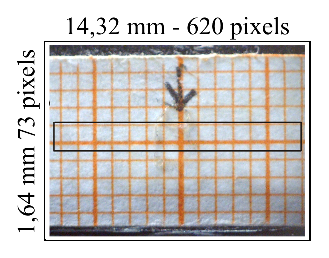
\includegraphics[scale=1.0]{eps/procedure_laser_BW_regua2.eps}} \qquad
%\subfigure[4 imagens superpostas]{
\includegraphics[scale=1.0]{eps/procedure_laser_BW_4frames_2.eps}} \qquad
%\subfigure[2000 imagens superpostas de %gotas]{\label{3figs-c}
\includegraphics[scale=1.0]{eps/procedure_laser_BW_2000_frames2.eps}}%
%\centering \caption{processo de registro de imagens na determina\c{c}\~{a}o do volume de amostragem.}
%\label{3figs}
%\end{figure}

\begin{figure}%
\centering
\subfigure[ ]{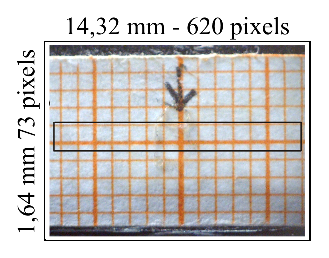
\includegraphics[scale=0.9]{eps/procedure_laser_BW_regua2.eps}} \qquad
\subfigure[ ]{
\includegraphics[scale=0.9]{eps/procedure_laser_BW_4frames_2.eps}} \qquad
\subfigure[ ]{\label{3figs-c}
\includegraphics[scale=0.9]{eps/procedure_laser_BW_2000_frames2.eps}}%
\centering \caption{ imagens do processo de calibra\c{c}\~{a}o, (a) papel milimetrado no centro da c\^{a}mara de nuvens; (b) got\'{\i}culas dentro da c\^{a}mara de nuvens; (c) resultado de 2000 imagens sobrepostas.}
\label{3figs}
\end{figure}

O valor de $i(y)$ de todos os \textit{pixels} iluminados ao longo de todo o feixe de luz LASER para cada altura \textit{y} (em \textit{pixels}) \'{e} mostrado na Figura \ref{grafico_diametro} e dado por



% MathType!MTEF!2!1!+-
% feqaeaartrvr0aaatCvAUfeBSjuyZL2yd9gzLbvyNv2CaerbuLwBLn
% hiov2DGi1BTfMBaeXatLxBI9gBaebbnrfifHhDYfgasaacH8srps0l
% bbf9q8WrFfeuY-Hhbbf9v8qqaqFr0xc9pk0xbba9q8WqFfea0-yr0R
% Yxir-Jbba9q8aq0-yq-He9q8qqQ8frFve9Fve9Ff0dmeaabaqaciGa
% caGaaeqabaaaamaaaOqaaiaadMgadaWgaaWcbaGaamyEaaqabaGccq
% GH9aqpdaaeWbqaaiaadEgacaGGOaGaamiEaiaacYcacaWG5bGaaiyk
% aaWcbaGaamiEaiabg2da9iaaicdaaeaacaWGTbGaeyOeI0IaaGymaa
% qdcqGHris5aOGaaiilaiaadMhacqGH9aqpcaaIWaGaaiilaiaac6ca
% caGGUaGaaiOlaiaacYcacaWGUbGaeyOeI0IaaGymaaaa!4ADE!
%\[
\begin{equation}
 \label{iy}
i(y)  = \sum\limits_{x = 0}^{m - 1} {g(x,y)}, \;\;\;y = 0,...,n - 1,
%\]
\end{equation}
em que \emph{m} e \emph{n} s\~{a}o  o n\'{u}mero de \textit{pixels} da imagem no eixo horizontal e vertical, respectivamente.


\begin{figure}[hbt]
\begin{center}
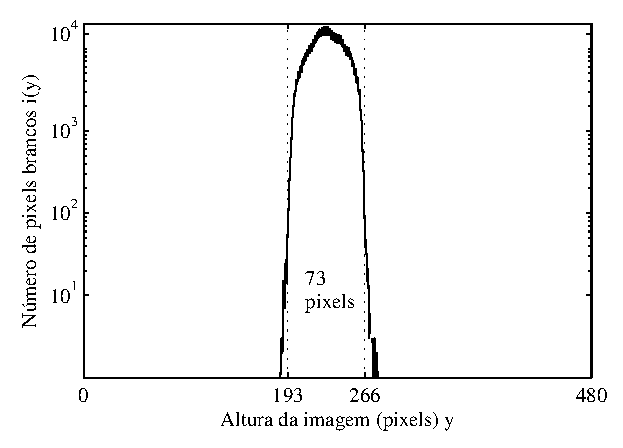
\includegraphics[scale=0.9]{eps/diametroLASER3.eps}\\
\end{center}
\centering \caption{\label{grafico_diametro}\hspace{-0.1em} gr\'{a}fico de distribui\c{c}\~{a}o de \textit{pixels} brancos (valor 1) ao longo da altura da imagem.}
\end{figure}


Nesse procedimento, considera-se como di\^{a}metro da luz LASER as regi\~{o}es iniciais e finais que cont\'{e}m pelo menos 1\% do n\'{u}mero m\'{a}ximo de ocorr\^{e}ncias de \textit{pixels} ativados (iluminados). Na Figura \ref{grafico_diametro} \'{e} apresentado um gr\'{a}fico com o n\'{u}mero de vezes em que um determinado \textit{pixel} \'{e} ativado dentro de um grupo composto por 2000 imagens utilizadas na constru\c{c}\~{a}o da Figura \ref{3figs} (c).

Assim sendo, o di\^{a}metro do LASER \'{e} de 73 \textit{pixels}. Com o objetivo de ter o maior volume de amostragem poss\'{\i}vel, assume-se como comprimento do LASER 620 \textit{pixels}. A partir da rela\c{c}\~{a}o \emph{pixels}/mil\'{\i}metros (43,29 \emph{pixels}/mil\'{\i}metro na horizontal e 44,50 \emph{pixels}/mil\'{\i}metro na vertical), obtida atrav\'{e}s da an\'{a}lise da imagem mostrada na Figura \ref{3figs}a e da altura e do comprimento em \emph{pixels} definidos anteriormente, obt\'{e}m-se o valor do volume de amostragem conforme a equa\c{c}\~{a}o \ref{eq3} $V_a$=30,27 $\pm$ 1,76 mm$^3$. O valor da incerteza do volume (1,76 mm$^3$) \'{e} calculado considerando-se uma propaga\c{c}\~{a}o de erros, em fun\c{c}\~{a}o de um posicionamento errado do papel milimetrado dentro da c\^{a}mara de nuvens no valor de $\pm$1,0 mm,  de uma incerteza de  $\pm$ 1 \emph{pixel} tanto no di\^{a}metro quanto no comprimento bem al\'{e}m de um poss\'{\i}vel erro de 0,05 mm no papel milimetrado, pois este foi aferido com um paqu\'{\i}metro com esta resolu\c{c}\~{a}o.


Uma vez descrito e caracterizado o CCNC-SDCC proposto, podem-se obter resultados de sua opera\c{c}\~{a}o e com isto permitir uma an\'{a}lise comparativa entre este CCNC-SDCC e um contador de part\'{\i}culas condens\'{a}veis (CPC).





